\chapter{Robot Using}

% 场景为操作和使用机器人的基本功能模块,编写一个新场景即可开始操作机器人。

Before describing how to create and edit a scene, let us first get familiar with the scene editor of Lebai Robot and learn how to drag-and-drop teach\footnote{Drag-and-drop teaching: The robot is dragged and driven by human hands. At the same time, the robot can reach a self­balanced running state under the condition of correctly setting the mass and center of mass of the end tool.} operation.

% \vspace*{-0.8em}

\section{Scene Editor}

You can program the robot in the scene editor, i.e., edit the scene.
% \vspace*{-0.2em}
\subsection{Editor Type}

The scene module provides two types of editors:

\newpage

% 乐白机器人的场景支持使用如下两种编辑器进行编程:
\begin{itemize}[leftmargin=6.5em]
	\item [Timeline Editor]

	A scene editor that is visualized, easy to use, and does not require a user to understand any logical relationships. This editor is suitable for beginners, since a user only need to add corresponding blocks\footnote{In the timeline editor, each operable independent element is called a {\it block}, and a collection of several action blocks can be packaged into a package.} in the timeline editor as needed to operate the robot (See \prettyref{fig:时间轴编辑器}).

	\begin{figure}[htb]
		\centering
		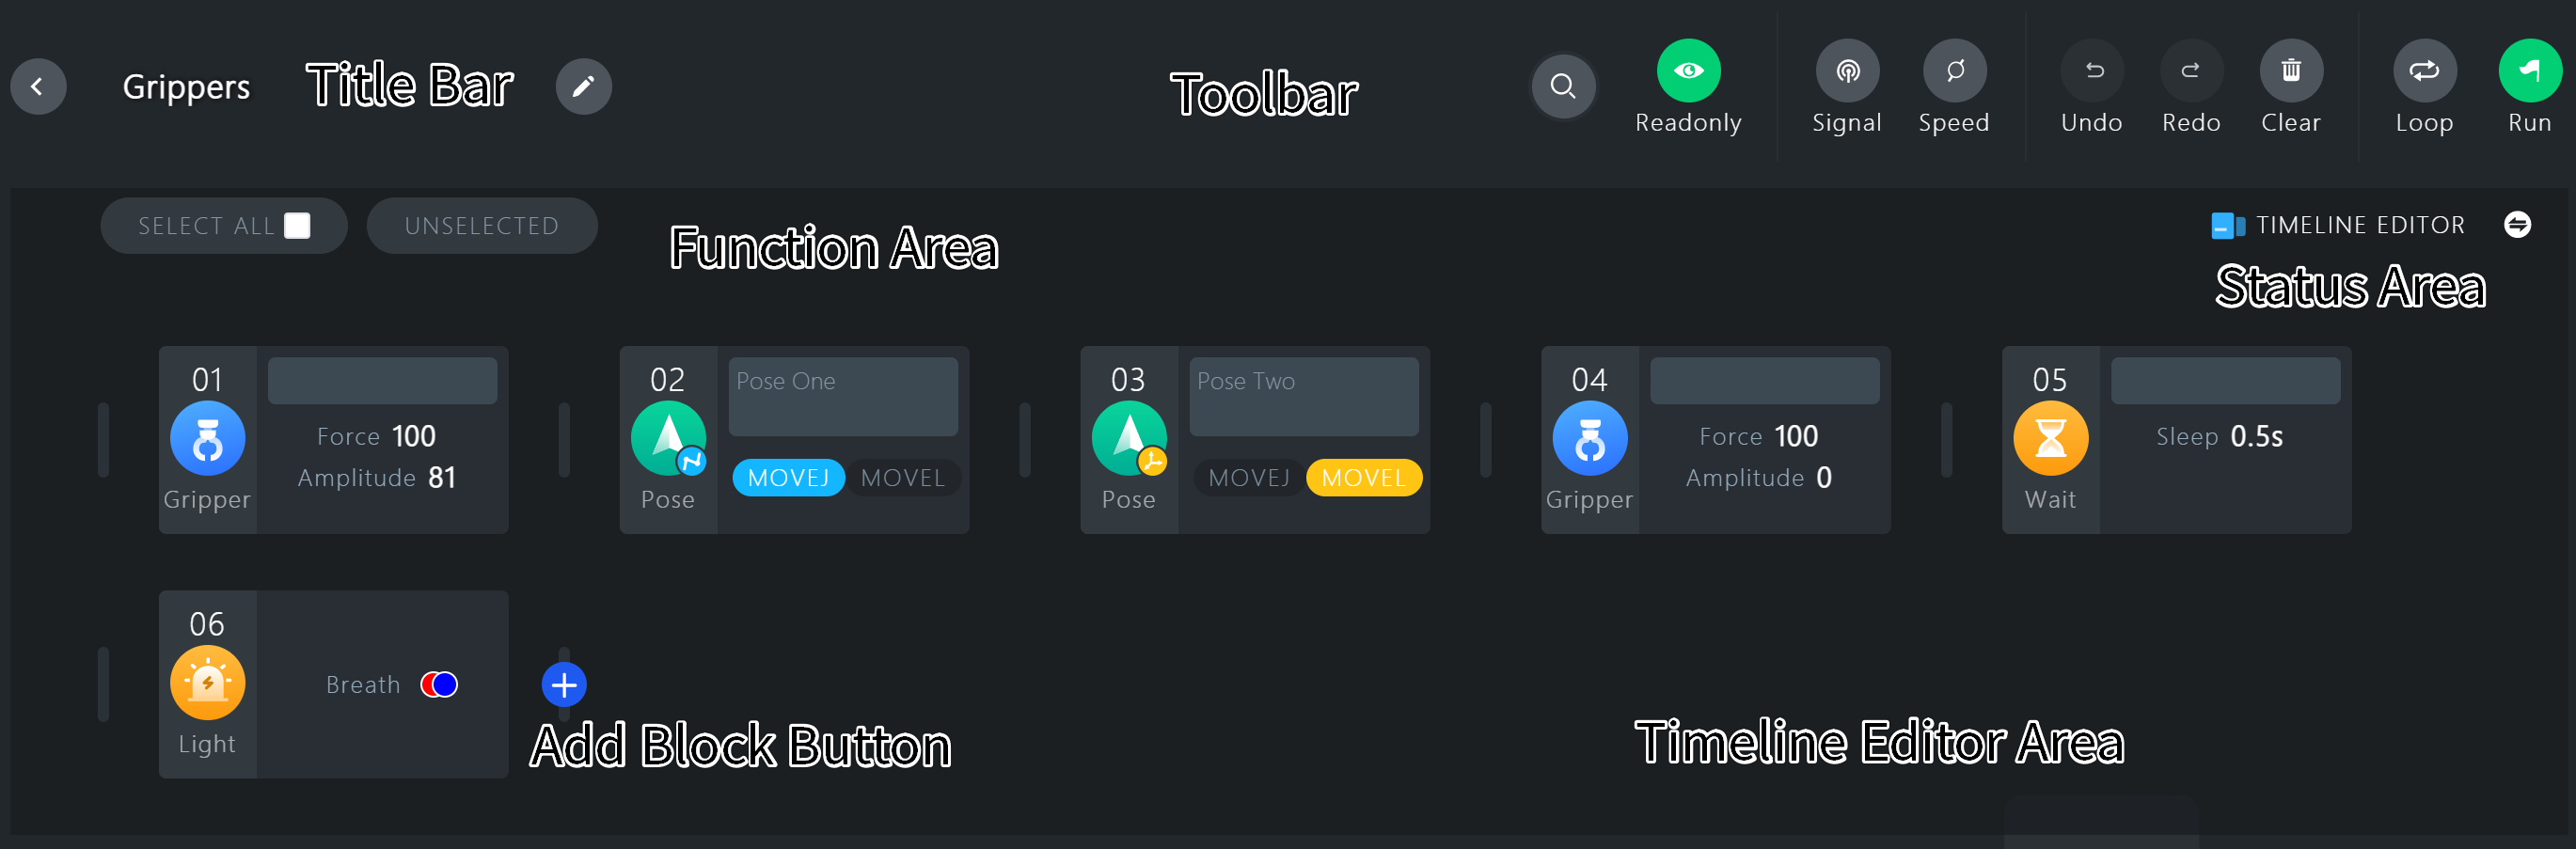
\includegraphics[width=\textwidth]{en/image/timeline.png}
		\caption{Timeline editor
		% \protect\footnotemark
		}
		\label{fig:时间轴编辑器}
	\end{figure}

	\newpage

	\item [Code Editor]

	A scene editor that is designed based on Lua language and supports complex operations. A scene editor that is designed based on Lua language and supports complex operations. It is suitable for users with a certain programming foundation and logical thinking. You can write codes to operate the robot (See \prettyref{fig:代码编辑器}).

		\begin{figure}[htb]
			\centering
		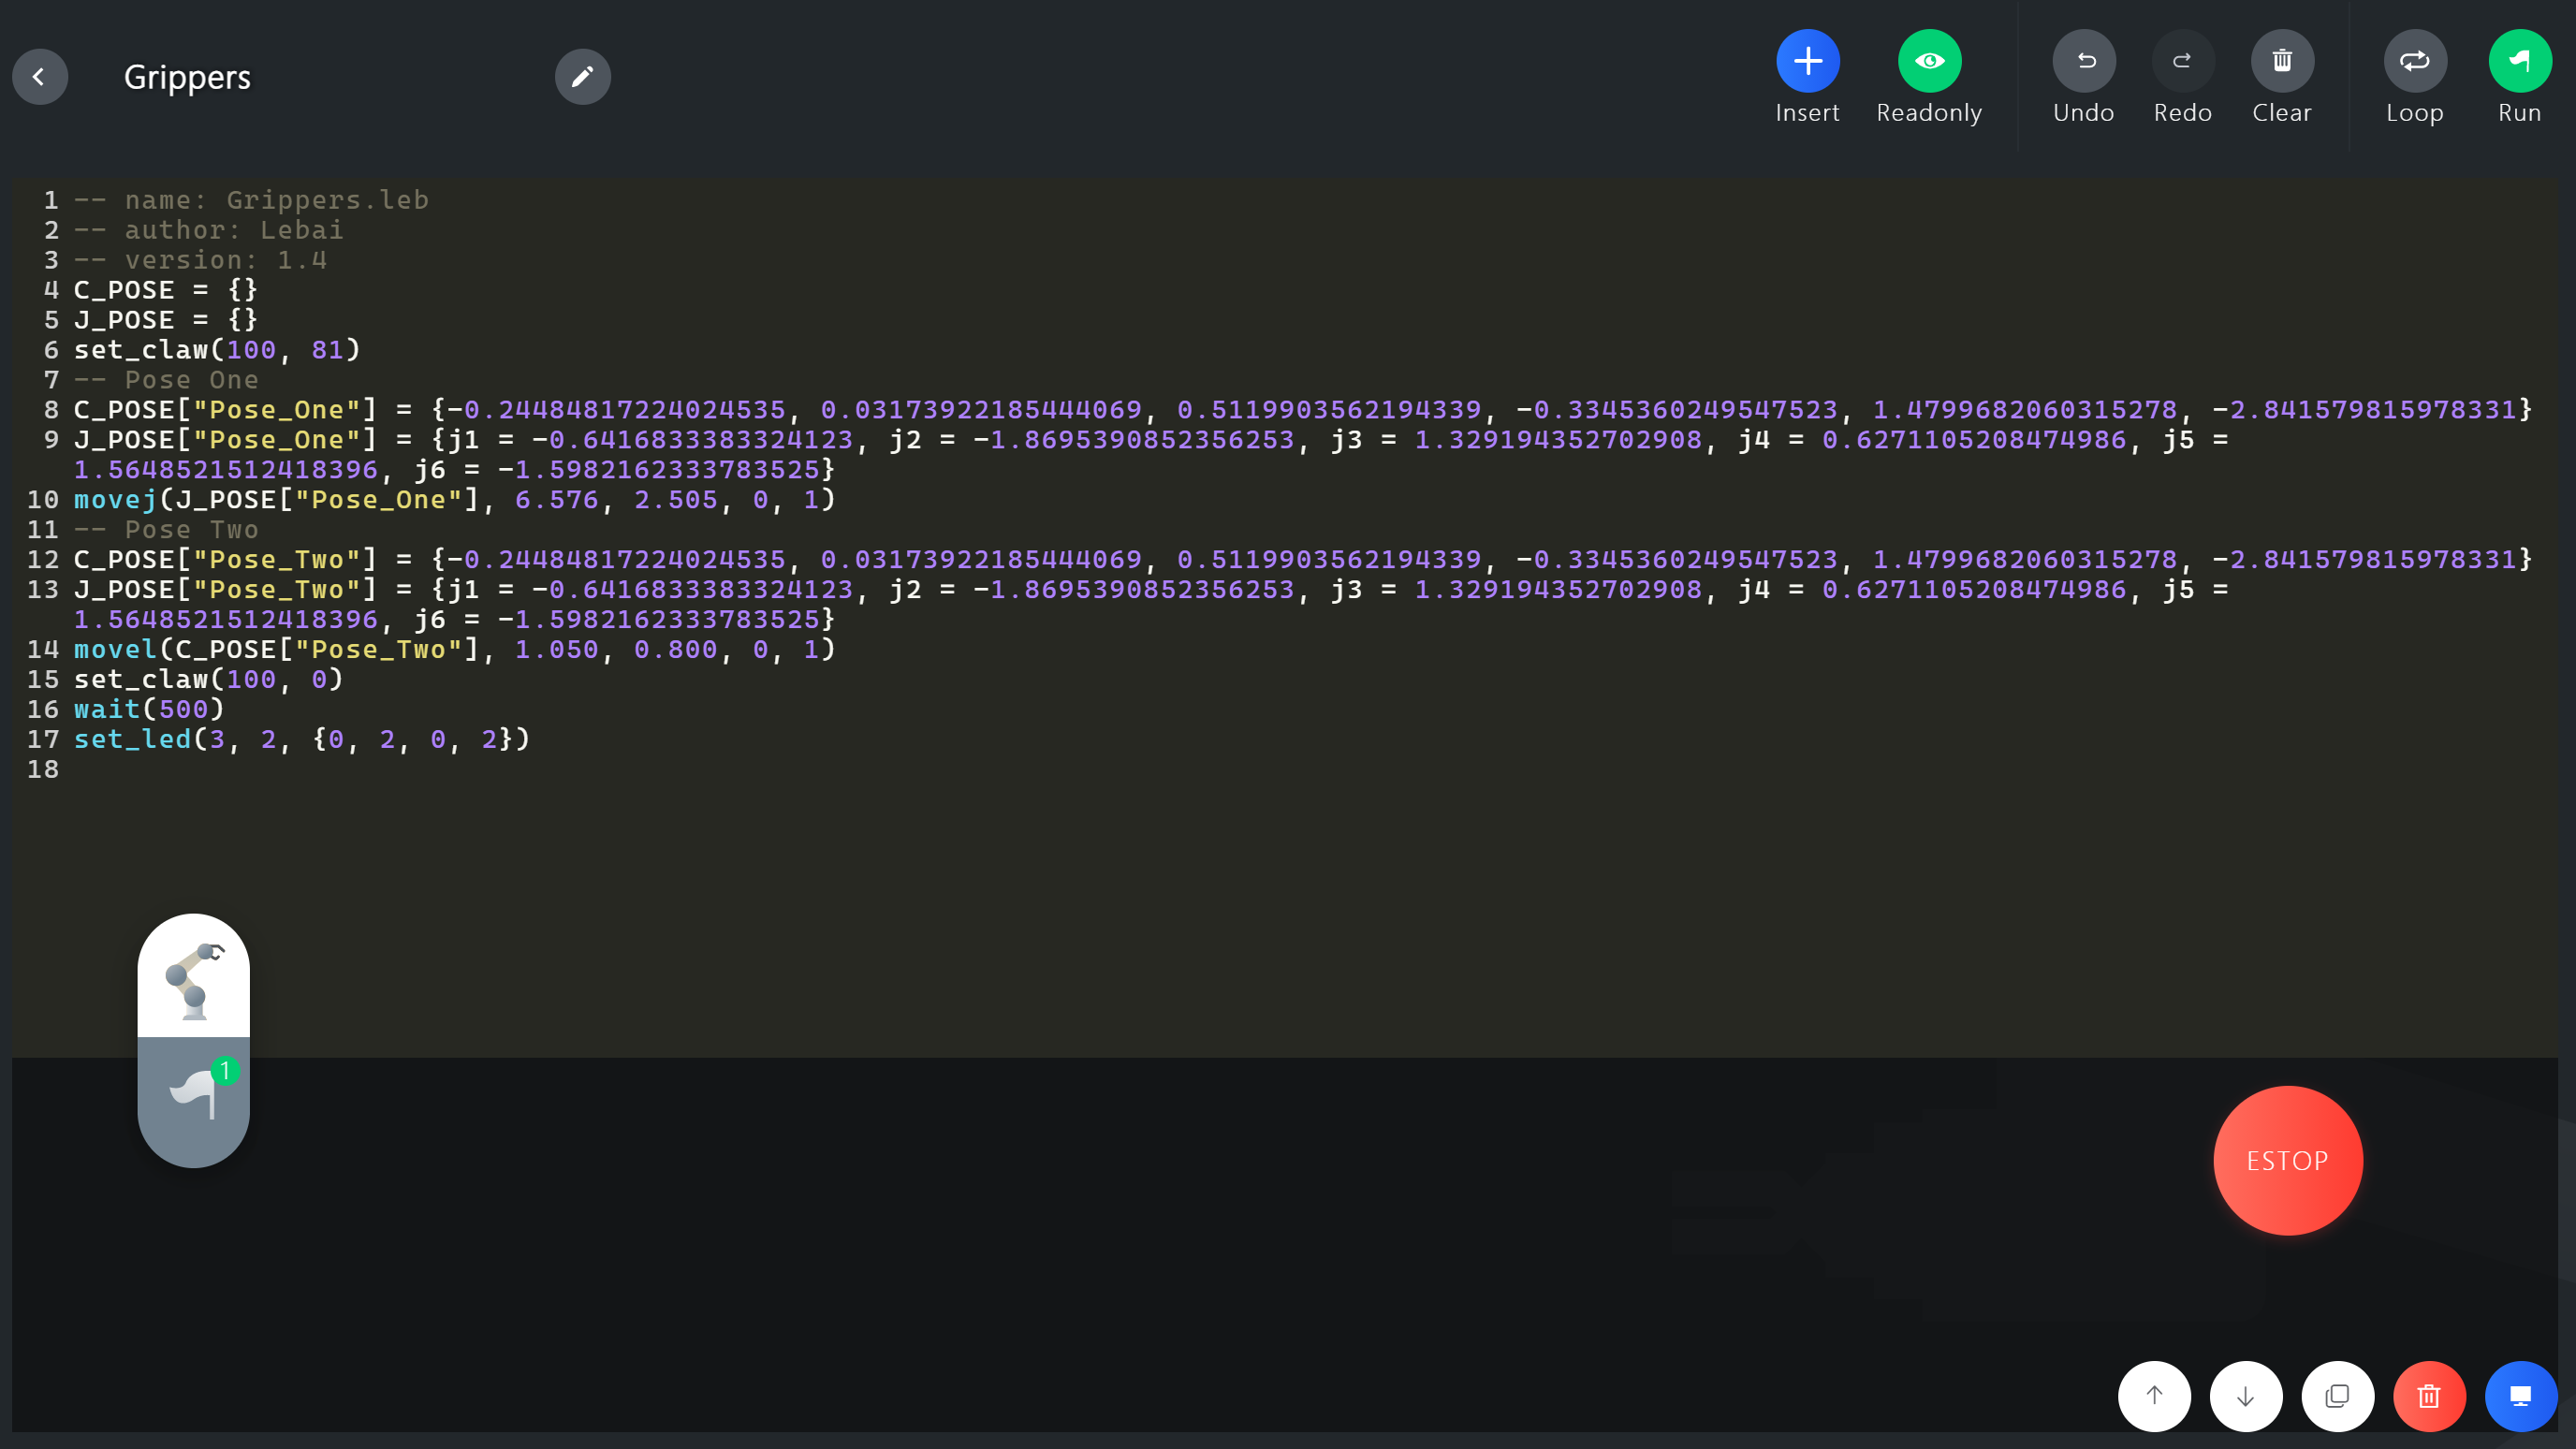
\includegraphics[width=\textwidth]{en/image/code.png}
		\caption{Code Editor}
		\label{fig:代码编辑器}
	\end{figure}
\end{itemize}

		% \vfill

			% \footnotetext{时间轴编辑器:以时间先后顺序展现机器人的顺序执行的动作列表,上海乐白机器人自主设计和研发的且拥有自主知识产权的专为机器人控制系统设计和研发的机器人场景编辑器。}

\clearpage

\subsection{Switch Editor Type}

The code editor is only available in the Expert Mode. The steps to switch from the Timeline Editor to the Code Editor are as follows:
\begin{enumerate}
\item Enter \mnu{SETTINGS}, click \mnu{OPERATION MODE}, or click the \colorbox{Black}{\icn{image/21.pdf}} button on the right side of the \mnu{Timeline Editor} in the status area to enter the operation mode selection page, select \mnu{Expert Mode} and click the \btn{SAVE} button in the upper right corner of the operation mode page.
\item Return to the previous scene that was being edited.
\item In the Timeline Editor, move the mouse to the \mnu{Timeline Editor} button, and select \mnu{Code Editor} in the pop­up menu to switch between the two editors.
\end{enumerate}

\begin{figure}[H]
	\centering
	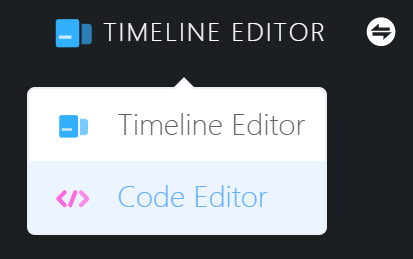
\includegraphics[height=2cm]{en/image/3-3.png}
	\caption{Switch Editor Type}
	\label{fig:切换编辑器类型}
\end{figure}

\info{When the editor of a scene is switched from the Timeline Editor to the Code Editor, it cannot be reversed back. Please \mnu{EXPORT} \footnote{See \prettyref{sec:导出场景}.} or \mnu{COPY} the scene you need to make a backup before operation.}

\vfill

\clearpage

% \subsection{类型图标说明}
% \begin{itemize}
% 	\item[\icn{image/43.pdf}] 在场景列表和场景编辑器页面出现此图标表示该场景为时间轴编辑器类型;
% 	\item[\icn{image/44.pdf}] 在场景列表和场景编辑器页面出现此图标表示该场景为代码编辑器类型。
% \end{itemize}

\section{Drag-and-Drop Teaching}
It is necessary to understand the drag-and-drop teaching method of Lebai robot before learning how to add pose blocks. There are two operation methods for drag-and-drop teaching for you to choose from:
\begin{itemize}
	\item Click the teaching icon \icn{image/36.pdf} in \LM to enable the teaching mode for the robot, drag the robot to the specified position, and click the teaching icon again to exit the teaching mode.
	\item Long press the robot's end convex button\footnote{See \prettyref{sec:硬件按钮}.} to enable the teaching mode for the robot. After dragging the robot to the certain position, release the robot's end convex button to exit the teaching mode.
\end{itemize}

\danger[WARNING]{Before use the drag-and-drop teaching, please make sure to set the mass and CoG of the end device\footnote{See \prettyref{sec:末端设备}.} correctly. Incorrect settings may result in accidental injury.\footnote{See \prettyref{sec:运行安全}.}}

\danger[WARNING]{In the teaching process, the rotation of joint angle should not exceed the safe range\footnote{See \prettyref{sec:运行安全}.}, otherwise it may cause the robot to stop suddenly or result in other faults.}

% \vfill

% \clearpage

\section{Scene Programming}
\subsection{Create A New Scene}
Click the \mnu{SCENE} button on the home page of \LM to enter the \mnu{SCENE LIST}, click the \btn[Info]{ADD SCENE} button on the right side of the toolbar on the page, and enter the scene name to complete the creation of a new scene.

\begin{figure}[ht]
	\centering
	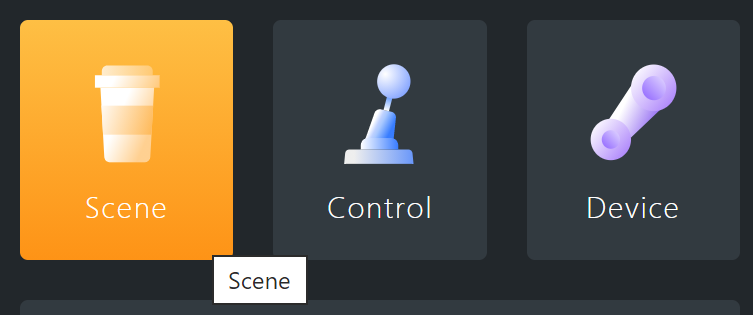
\includegraphics[height=2cm]{en/image/3-4.png}
	\caption{Scene entrance}
	\label{fig:场景入口}
\end{figure}

\subsection{Add A Block}

The Timeline Editor supports the following block types:
\begin{itemize}
\item Position
\item Gripper (Claw)
\item Wait
\item Notification
\item Digital I/O
\item Analog I/O
\item Semaphore
\item Payload
\end{itemize}

Click the Add Block button \icn{image/plus.pdf} in the Timeline Editor to pop up the \nameref{fig:添加动作块弹出框}, as shown in \prettyref{fig:添加动作块弹出框}.

\begin{figure}[ht]
	\centering
	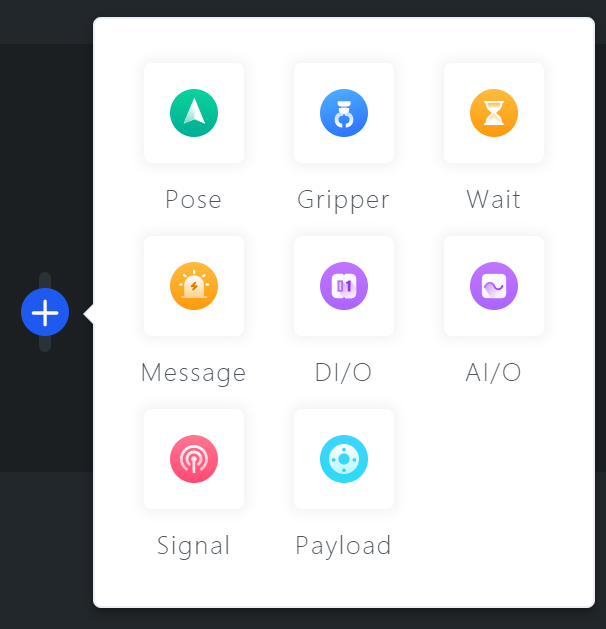
\includegraphics[width=5cm]{en/image/3-5.png}
	\caption{Choose block type}
	\label{fig:添加动作块弹出框}
\end{figure}

The following chapters describe the usage of different block types in turn.

\subsubsection{Pose Block}
Position\footnote{The ``position'' mentioned in {\ThisBook} consists of robot pose and posture data. In the subsequent content of this document, unless ``pose and posture'' is explicitly mentioned, all ``positions'' refer to the pose and posture of the robot.} is the core control module in robot control. In the Timeline Editor, you only need to add the pose blocks according to the following tutorial to make the robot move according to the predetermined pose and action.
\paragraph{Add position}
There are two ways to add a pose in the Timeline Editor for you to choose from:
\begin{itemize}
	\item Add Block button \icn{image/plus.pdf} in the editing area of the Timeline Editor, select the \mnu{Position}, enter the pose name in the open \nameref{fig:添加位置对话框} (as shown in \prettyref{fig:添加位置对话框}), and click the button to save the current pose of the robot in a new pose block\footnote{The ``block'' refers to the smallest visual editing module in the Timeline Editor. A ``module'' represents a type of actions which includes pose and I/O.}.
	\item Double­click the convex button at the end of the robot, and the system will save the current pose of the robot in a new pose block.
\end{itemize}

\begin{figure}[ht]
	\centering
	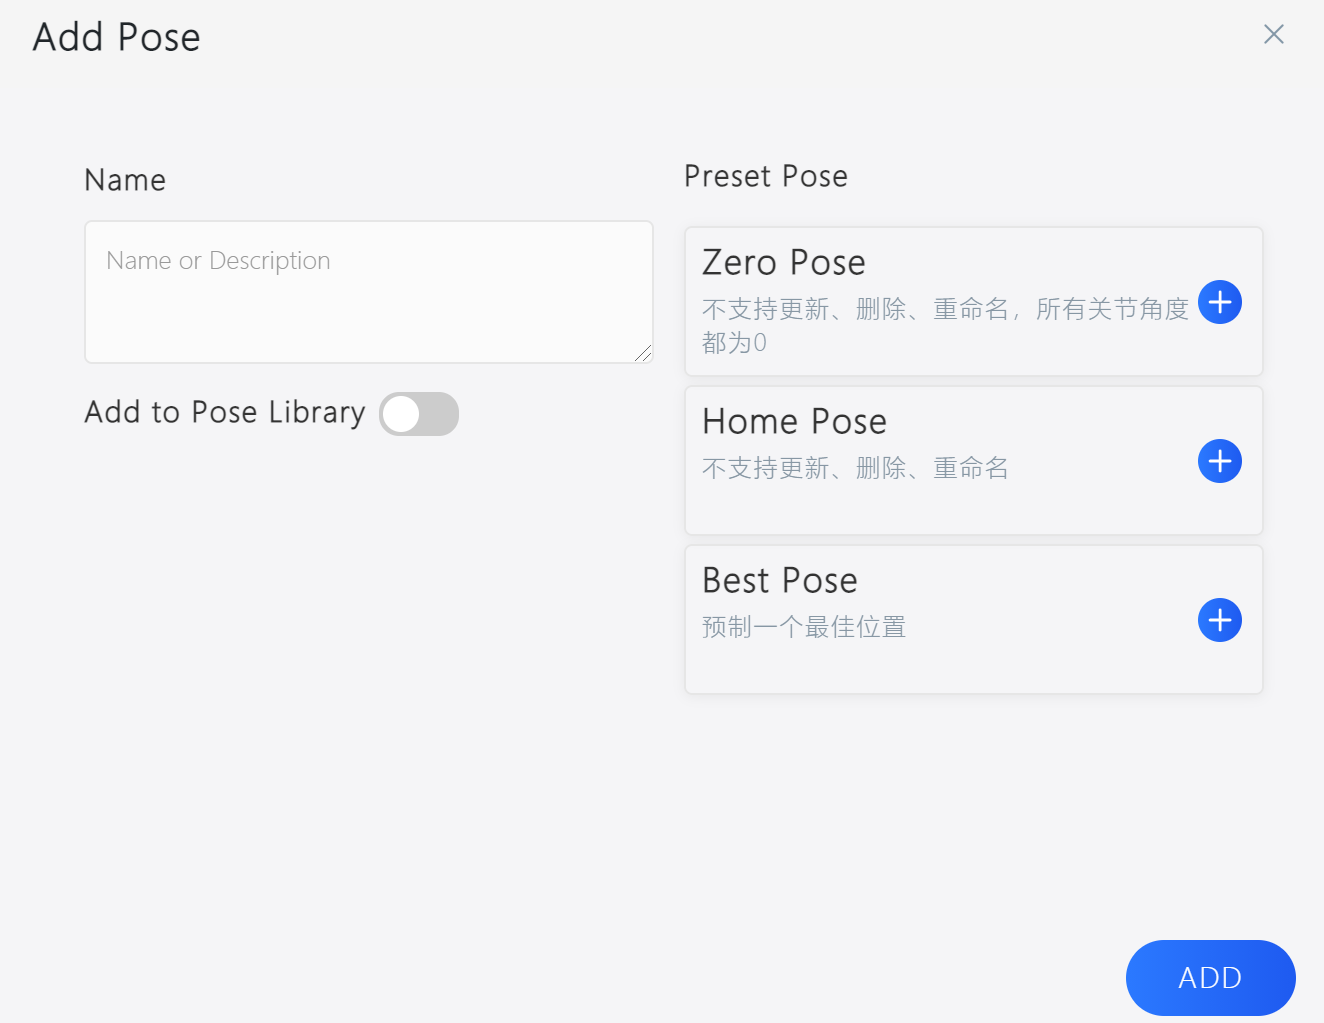
\includegraphics[height=6cm]{en/image/3-6.png}
	\caption{Dialog of add position}
	\label{fig:添加位置对话框}
\end{figure}

By combining the drag-and-drop teaching and the above method of adding pose blocks, you can add the desired pose blocks according to your needs (as many as you want) until the scene editing is complete.

\paragraph{Edit position}
\label{sec:编辑位置}
As shown in \prettyref{fig:位置块焦点状态}, place the cursor on the pose block to make the current pose block in focus.

\begin{figure}[ht]
	\centering
	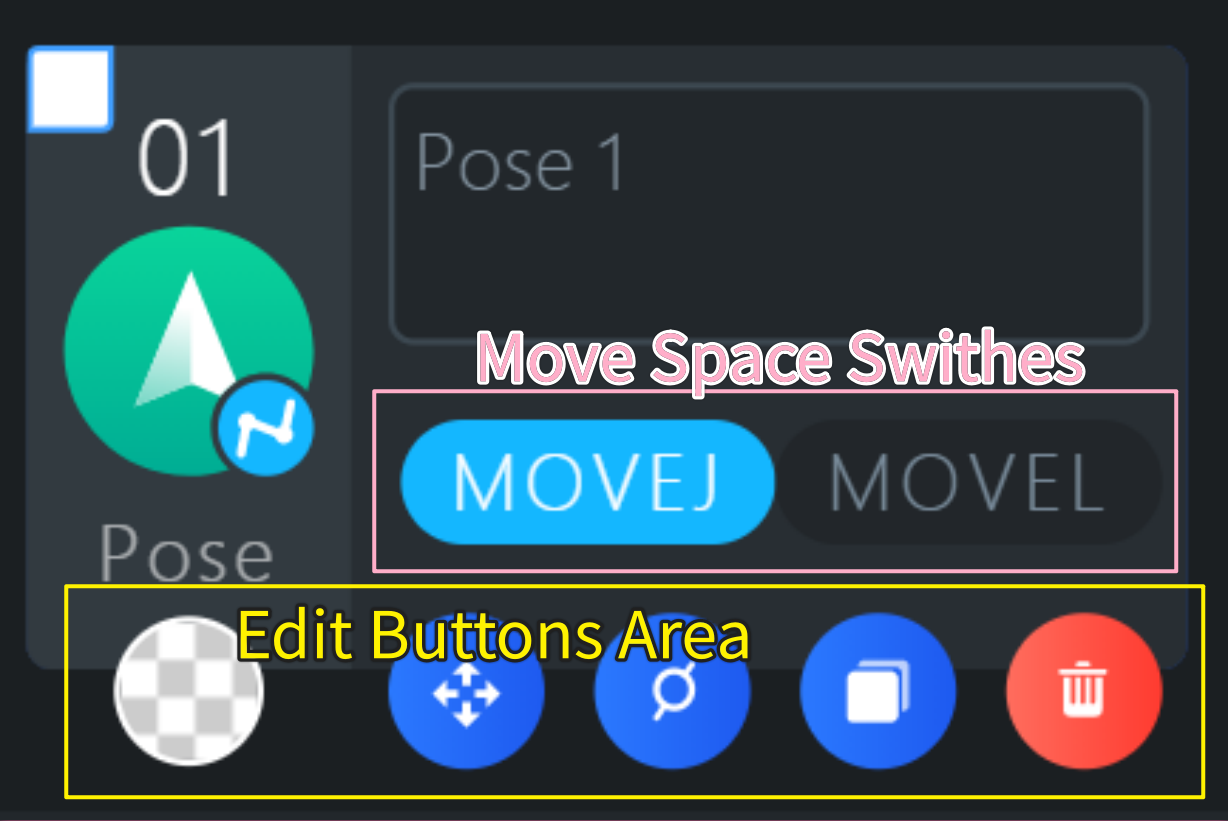
\includegraphics[height=3.5cm]{en/image/pose-block.png}
	\caption{The focal state of the pose block}
	\label{fig:位置块焦点状态}
\end{figure}

The two buttons in the trajectory type switching area are used to switch between joint space movement (movej) and Cartesian space linear movement (movel).

\newpage

\begin{itemize}
	\item[\icn{image/ic_joint.pdf}] Represents the movement in joint space\footnote{Joint space: the robot motion space described with the angle of each joint of the robot.}.
	\item[\icn{image/ic_line.pdf}] Represents the linear motion in Cartesian space\footnote{Cartesian space: The full name is Cartesian coordinate system space, which is the rectangular coordinate system space we commonly use.}.
\end{itemize}

The buttons in the edit operation button area are:

\begin{itemize}
\item [\quad] {\sffamily\bfseries Style}: The background color of the block can be changed\footnote{The color of the {Style} button is consistent with the background color of the block. When a block is selected, the block will be highlighted with this color as the background. In particular, the style is transparent by default, and the highlighted back­ ground color selected by the block is blue. The Style, Copy, and Delete buttons are common buttons in the block operation button area.}.
\item [\icn{image/ic_adjust.pdf}] {\sffamily\bfseries Fine-tuning}: Fine­tune and update the location data stored in the current location block.
\newpage
\item [\icn{image/ic_a_v.pdf}] {\sffamily\bfseries Speed and Acceleration Time}: Adjust the speed and acceleration time of the pose block\footnote{The acceleration time is inversely proportional to the acceleration. The greater the acceleration, the shorter the acceleration time; while the shorter the acceleration time, the longer the acceleration time.}.
\item [\icn{image/ic_copy.pdf}] {\sffamily\bfseries Copy}: Copy a current block.
\item [\icn{image/ic_delete.pdf}] {\sffamily\bfseries Delete}: Delete the current block.
\end{itemize}

\paragraph{Fine-tuning}
\label{sec:微调}
When editing a scene, the pose in the motion track needs to be fine­tuned precisely by applying fine-tuning to individual positions. Select the Fine­tuning icon, and the page will automatically jump to the fine­tuning page.

% 微调页面中虚的机器人和实的机器人底座重叠展示,其中虚的机器人表示当前位置块存储的目标位置,实的机器人表示机器人当前位置。
When the current \mnu{ACTUAL POSITION} of the robot is inconsistent with the \mnu{TARGET POSITION} stored in the pose block, a blur robot icon and a solid robot icon will appear in the fine­tuning page. The blur one represents the target pose stored in the current pose block, and the solid one represents the current actual pose of the robot.

You can switch between the actual pose \icn{image/position.pdf} and the target pose \icn{image/saved.pdf} using switch button to view the values of the target pose and the actual position.

\subparagraph{Coordinate space fine-tuning}

\begin{figure}[ht]
	\centering
	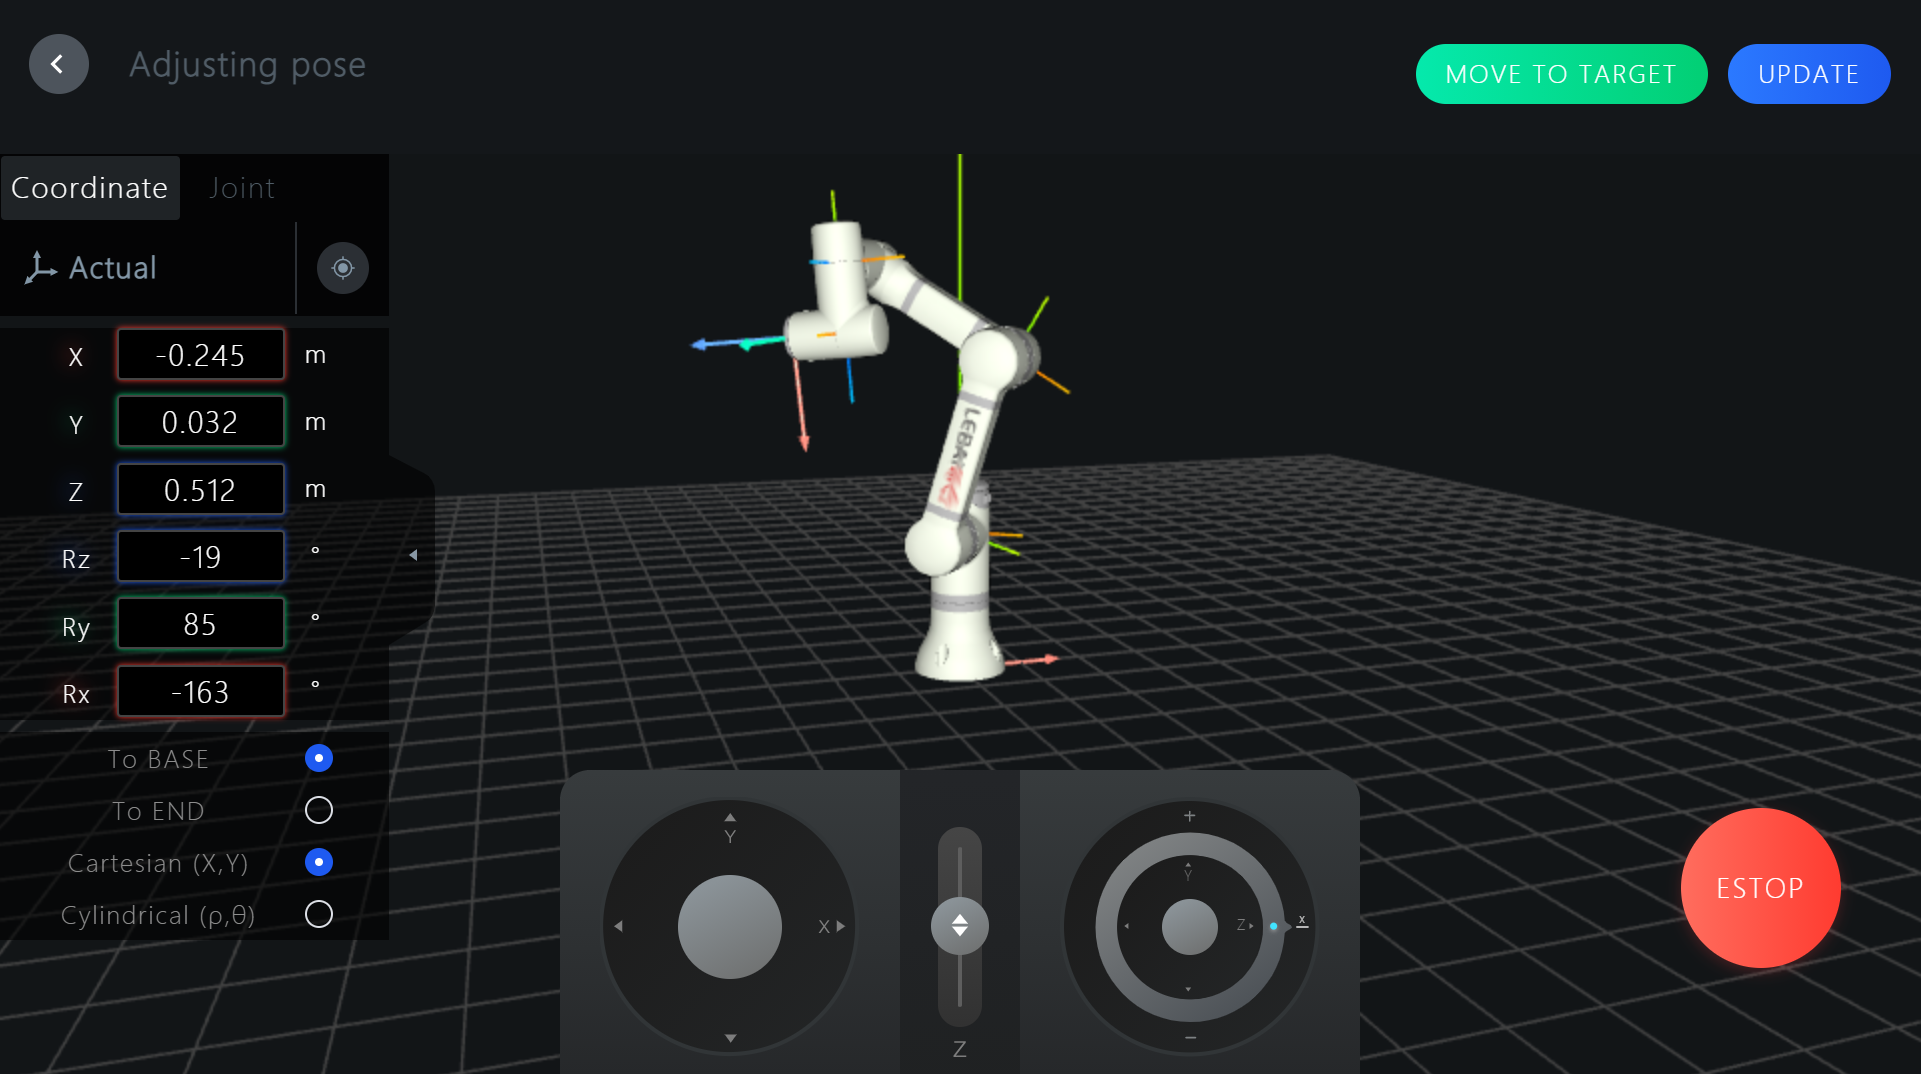
\includegraphics[width=\textwidth]{en/image/coor.png}
	\caption{Coordinate space fine-tuning}
	\label{fig:坐标空间微调}
\end{figure}

Different coordinate system representation methods can be selected during fine­tuning:
\begin{itemize}
	\item When ``relative to the Base'', the rectangular coordinate system or cylindrical coordinate system can be used.
	\item When ``relative to the End'', only Cartesian coordinate system is supported.
\end{itemize}

\begin{figure}[ht]
	\centering
	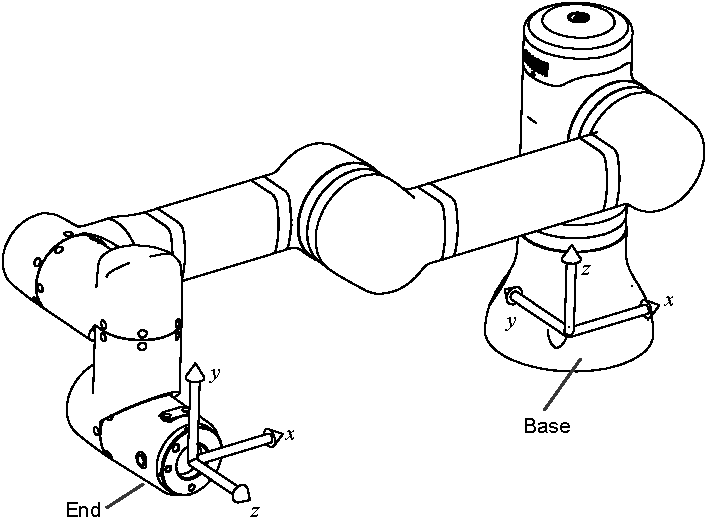
\includegraphics[height=6cm]{en/image/fine_tuning_coordinate.pdf}
	\caption{Coordinate to the base or the end}
	\label{fig:坐标空间示意图}
\end{figure}

When the reference coordinate system is \mnu{To BASE}, it means that the center of the robot base is taken as the origin of the coordinate system.

By selecting the Cartesian coordinate system as the adjustment method, and entering the pose $(X, Y, Z)$ or posture $(R_z, R_y, R_x)$\footnote{The posture of Lebai robot in Cartesian space (Cartesian coordinate system space) adopts EulerZYX notation, please refer to related robot basic books or tutorials. The posture $(R_z, R_y, R_x)$ can also be described as $(\alpha, \beta, \gamma)$.} value in the pose information display box on the fine­tuning page, the robot will automatically move to the pose you choose. You can also operate the robot by pulling the levers in all directions at the bottom of the screen. When the lever is released, the fine adjustment stops. Click the \btn{UPDATE} button to complete the fine adjustment.

Lebai robot uses $Z\textrm{-}Y\textrm{-}X$ Euler angle (EulerZYX) to describe the posture of the end of the robot, that is, first rotate the $R_z$ angle around the $Z$ axis of the coordinate system, then rotate the $R_y$ angle around the $Y$ axis of the rotated coordinate system, and finally rotate around the $X$ axis of the coordinate system by the $R_x$ angle twice.

Select the cylindrical coordinate system\footnote{The X­Y plane of the cylindrical coordinate system is the polar coordinate system. The point $P(x, y, z)$ in the rectangular coordinate system is represented as $P'(\rho, \theta, z)$ in the cylindrical coordinate system, where $\rho=\sqrt{x^2+y^2}$,$\theta=\arctan\frac{y}{x}$.} , the left adjustment dial will change from adjustment $(X, Y)$ to adjustment $(\rho, \theta)$.

When the reference coordinate system is selected as \mnu{To END} (without adding TCP\footnote{See \prettyref{sec:TCP设置}.}), the center of the robot flange is used as the origin of the coordinate system, and the rectangular coordinate system is used as the adjustment method. Enter the pose or posture on the fine adjustment page or set the value or pull the lever at the bottom of the screen. After the robot automatically moves to the specified position, click \btn{UPDATE} to complete the fine adjustment of the position.

\subparagraph{Joint space fine-tuning}
Click on the \mnu{Joint Space} at the top left of the fine­tuning page, and enter the angle value of joint 1 to joint 6, then the robot will automatically reach the specified position. Or pull the levers in all directions at the bottom of the screen to operate the robot. When the lever is released, fine­tuning stops. Click \btn{UPDATE} to complete Fine adjustment of position.

\begin{figure}[ht]
	\centering
	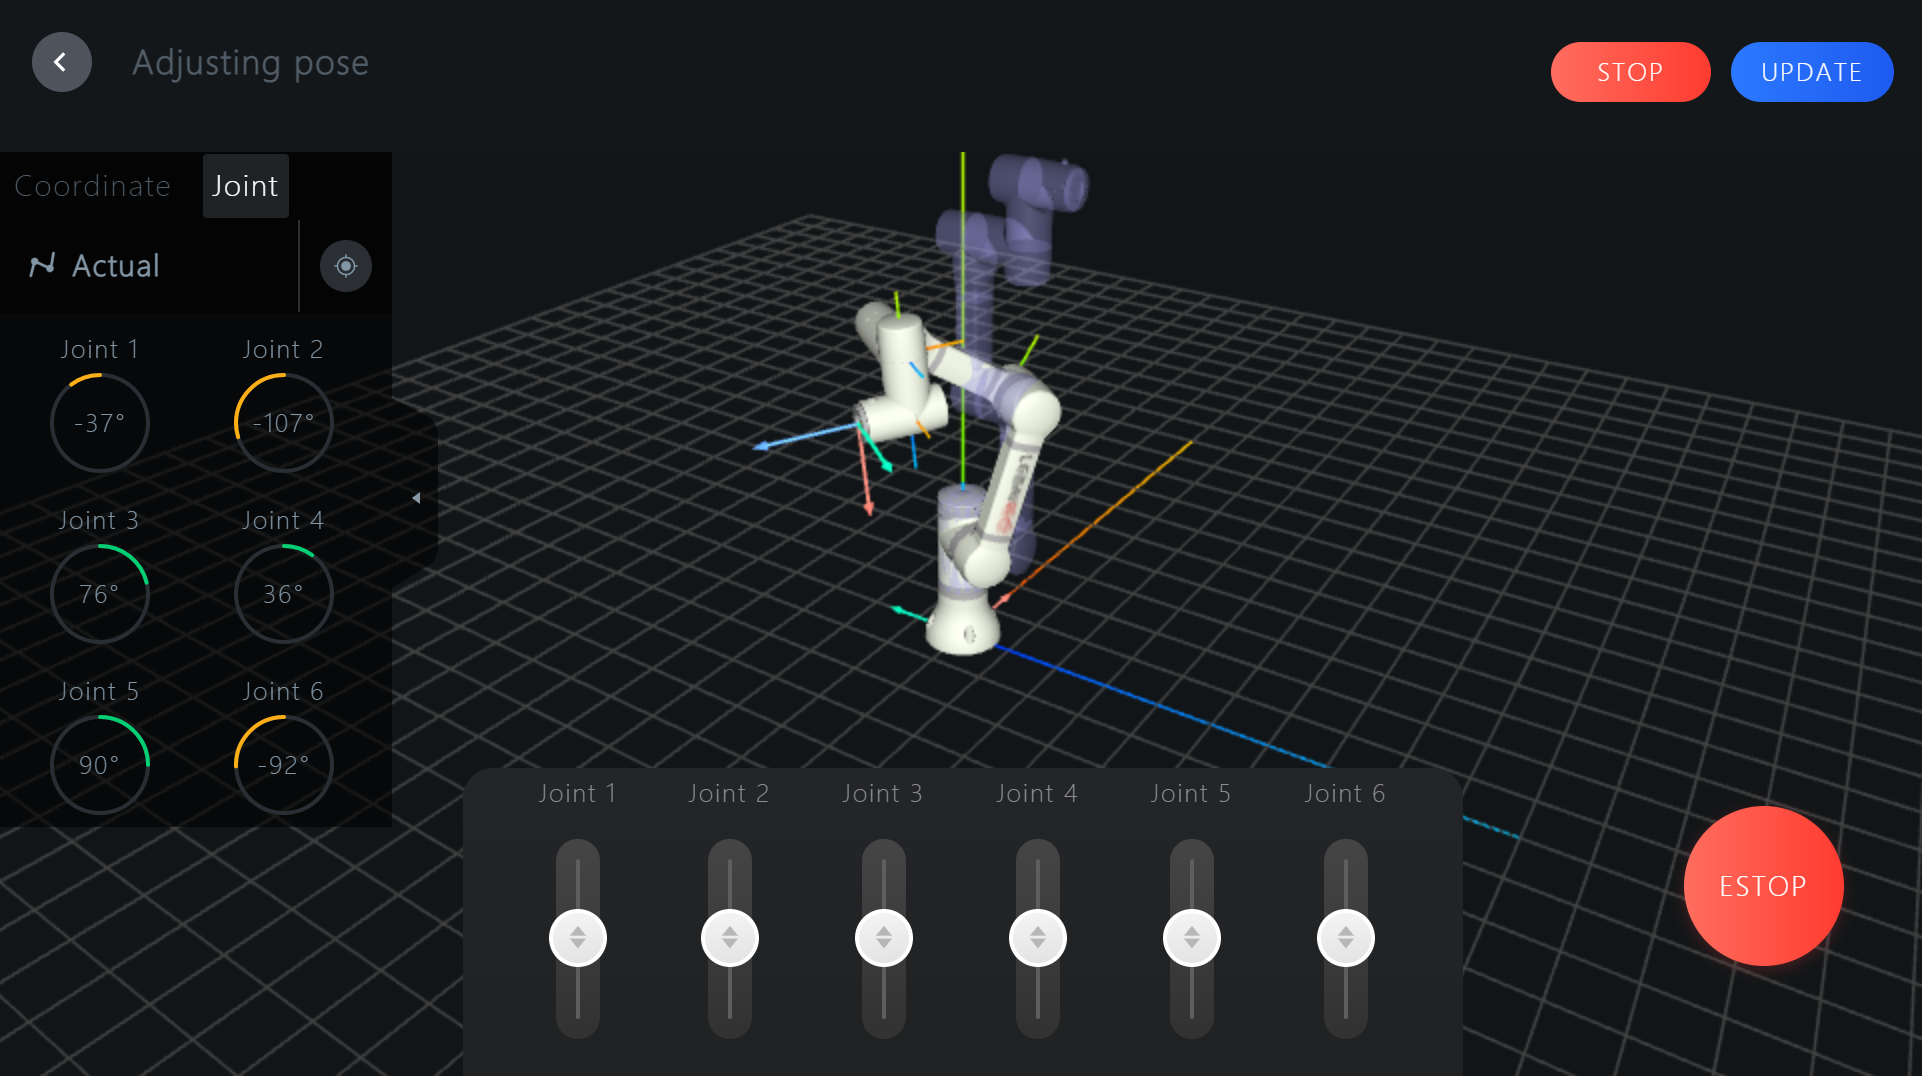
\includegraphics[width=\textwidth]{en/image/joints.png}
	\caption{Joint space fine-tuning}
	\label{fig:关节空间微调}
\end{figure}

\paragraph{Speed and acceleration time}
Speed and acceleration time are modified for the current scene or the speed ($v$) and acceleration ($a$) of a single location block. The horizontal axis corresponds to the acceleration time. The vertical axis corresponds to the speed. The closer the vertical axis is to the origin, the lower the speed.

\begin{figure}[ht]
	\centering
	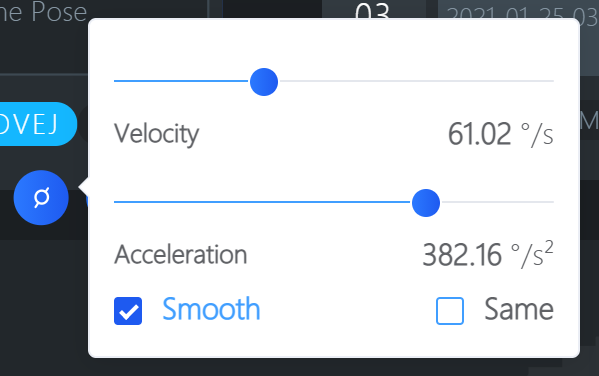
\includegraphics[height=4cm]{en/image/3-11.png}
	\caption{Speed and acceleration time control}
	\label{fig:速度控件}
\end{figure}

To adjust the speed and acceleration time, the user can do it globally\footnote{See \prettyref{sec:速度和加速时间}.} on the toolbar of the scene editor13, or individually for each pose block.

Click the pose block \icn{image/ic_a_v.pdf} button to pop up the \nameref{fig:速度控件}. The icon \icn{image/lock.pdf} in the upper right corner is the synchronization lock between the current pose block and the information about global speed and acceleration time on the editor toolbar. When a new pose is added to the scene, the global lock of the speed and acceleration time control of the pose block is locked by default, which means it is consistent with the global speed and acceleration time of the current scene. When the user drags a drag point to adjust the horizontal or vertical axis of the control and changes the speed and acceleration time, the global lock will be unlocked, that is, the pose block uses the speed and acceleration time specified by yourself and no longer uses the global speed and acceleration time parameter values. You can click the icon \icn{image/unlock.pdf} again to lock Synchronization lock, then the pose block will keep the parameter value consistent with the global speed and acceleration time.

The smooth function mainly refers to that the robot control system automatically optimizes the best path and passes through the target pose of the current pose block without stopping, making the action continuity better and the moving time shorter when there are multiple adjacent pose blocks. higher efficiency. When the smoothing function is turned on, there will be no obvious slowdown and stop when the robot moves between the two blocks.

After adding pose blocks, if you don't need to add other types of blocks, you can move to \prettyref{sec:运行场景}.

\subsubsection{Gripper Block}

\begin{figure}[htb]
	\centering
	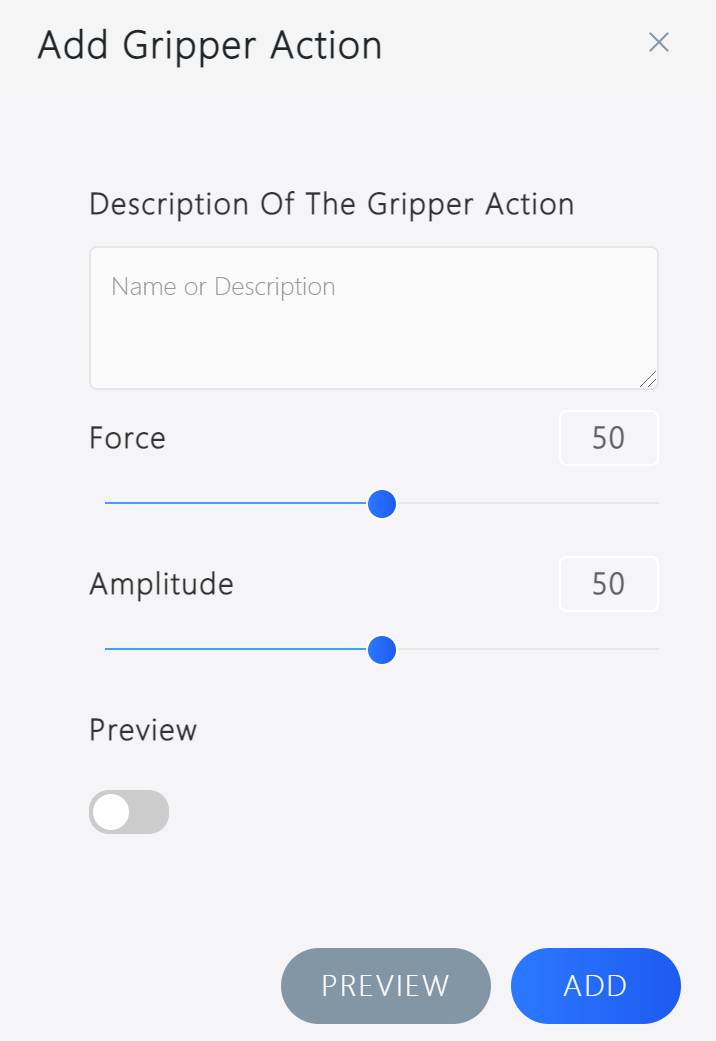
\includegraphics[height=6cm]{en/image/3-12.png}
	\caption{Dialog of adding gripper block}
	\label{fig:添加手爪动作对话框}
\end{figure}

Select \mnu{Gripper} in the \nameref{fig:添加动作块弹出框}, and the \nameref{fig:添加手爪动作对话框} will pop up (See \prettyref{fig:添加手爪动作对话框}). Enter a description of the Gripper action and set the strength and amplitude. If you need to preview the opening and closing effect of the Gripper, please turn on the \mnu{Preview} switch (real­time preview) or click the \btn[Info]{PRVIEW} button (manual preview). After confirming the effect is correct, click \btn{ADD}.

\subsubsection{Wait Block}
Select \mnu{Wait} in the \nameref{fig:添加动作块弹出框} enter the number of seconds to wait.
\subsubsection{Notification Block}
Select \mnu{Notification} in the \nameref{fig:添加动作块弹出框}. Notifications are divided into light board prompts and pop­up prompts. The light board prompts are as follows:
\begin{itemize}[leftmargin=10em]
\item[Off] The light board turns off the display;
\item[Always on] The light board keeps the specified color always on;
\item[Breathing] The light board breathes in the specified color;
\item[Evenly rotating] The light board displays in evenly distributed rotation between 2 or 4 designated different colors;
\item[Rotate with the same color] The light board displays rotating in a certain color;
\item[Flashing] The light board flashes in a certain color.
\end{itemize}
\subsubsection{Digital I/O Block}
Select \mnu{Digital I/O} in the \nameref{fig:添加动作块弹出框}. In the pop­up Add dialog box, the top tab corresponds to the operation type of the digital I/O. The digital I/O block supports three types of operations:
\begin{itemize}[leftmargin=4.5em]
\item[Read] Read the input value of a digital I/O port;
\item[Wait] When the block is executed, it will stay and wait for the value of a certain digital I/O to become the selected value;
\item[Set] Set the output value of a certain digital I/O port.
\end{itemize}

There are three types of digital I/O ports: control box I/O, flange I/O and external I/O (if any).

% \clearpage

Click \btn{ADD} to complete the insertion of a simulated I/O block.
% \begin{itemize}
% 	\item 控制箱I/O
% 	\item 法兰盘I/O
% 	\item 外置I/O
% \end{itemize}

% \info{运行任务前请确认要使用的I/O输入输出电气连接正常。}

% \vfill

\info{Before running the task, make sure that the input and output electrical connections of the digital I/O are operational.}

% \vfill

\subsubsection{Analog I/O Block}
Select \mnu{Analog I/O} in the \nameref{fig:添加动作块弹出框}. In the pop­up Add dialog box, the top tab corresponds to the operation type of the analog I/O. The analog I/O block supports three types of operations:
\begin{itemize}[leftmargin=4.5em]
\item[Read] Read the input value of a analog I/O port;
\item[Wait] When the block is executed, it will stay and wait for the judgment condition of a certain analog I/O value matching the selected value;
\item[Set] Set the output value of an analog I/O port.
\end{itemize}

There are only two types of analog I/O ports: control box I/O and external I/O (if any). The flange has no analog I/O ports.

Click to \btn{ADD} complete the insertion of a simulated I/O block.

% \vfill

\info{Before running the task, make sure that the input and output electrical connections of the analog I/O are operational.}

% \vfill

% \clearpage

\begin{figure}[ht]
	\centering
	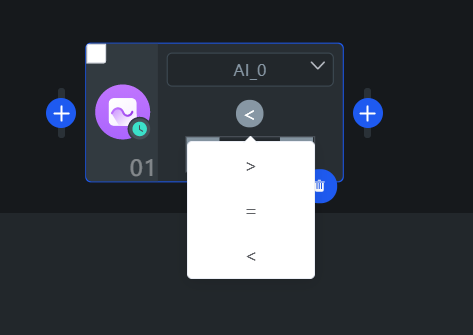
\includegraphics[height=3cm]{en/image/3-13.png}
	\caption{Analog I/O judgment conditions}
	\label{fig:模拟IO判断条件}
\end{figure}

Under the waiting operation type, there are three judgment conditions: >, =, and <. Click the waiting condition button of a waiting analog I/O block (as shown in \prettyref{fig:模拟IO判断条件}) to edit the corresponding judgment conditions.

\subsubsection{Payload Block}
Select \mnu{Payload} in the \nameref{fig:添加动作块弹出框}, and enter the load mass or CoG that needs to be modified in the Add Playload dialog box. This function is used to edit the mass and CoG of the load at runtime.

\danger[WARNING]{When the robot is installed with a end-effector, and the end-effector has functions such as picking and placing items, it is necessary to insert an block corresponding to the change in mass and CoG in the end load after picking and placing in the corresponding pose of the Timeline Editor. If not set normally, there might be reduction in the life of the corresponding parts of the robot, and false alarms in collision detection might result.}

\danger[WARNING]{When adding a Playload configuration, the mass and CoG settings must be as consistent as the end-effector quality. If you need to replace or remove the end-effector, you must edit the load parameters or disable the corresponding end device accordingly, otherwise acci­ dental injury might result.}

\subsection{Toolbar}
The toolbar of the Timeline Editor can provide functions such as searching, editing, operation and execution for the scene.

\begin{figure}[ht]
	\centering
	
\includegraphics[width=\textwidth]{en/image/3-14.png}
	\caption{Timeline editor toolbar}
	\label{fig:时间轴编辑器工具栏}
\end{figure}

\subsubsection{Change the Scene Name}
Click the Edit button \icn{image/ic_toolbar_edit.pdf} behind the title text of the toolbar to edit the scene name in the pop­up Scene modification dialog box.
\subsubsection{Search}
Click the Search button to expand the block search box.

\begin{figure}[ht]
	\centering
	
\includegraphics[width=\textwidth]{en/image/3-15.png}
	\caption{Expanded block search box}
	\label{fig:展开的动作块搜索框}
\end{figure}

In the expanded state of the search box, click the icon \icn{image/all.pdf} on the left side of the search box to search based on the block type in the pop­up box quickly. At the same time, you can also use the keywords entered in the text input box to search for the blocks of the corresponding type or all types that match the keyword.

% \vfill

\subsubsection{Semaphore}
The semaphore is temporarily not available in \LM~v2.1.

% \vfill

\subsubsection{Speed and Acceleration Time}
\label{sec:速度和加速时间}
The Speed and acceleration time on the toolbar are the configuration entries for the global speed and acceleration time of the current scene. When the speed and acceleration time adjustment operations of a single pose block mentioned in \prettyref{sec:编辑位置} are not applicable, all pose blocks in this scene use the global configuration of speed and acceleration time.

% \vfill

\subsubsection{Undo/Redo}
When you deleted an block by mistake or performed a wrong operation, you can click the undo button \icn{image/ic_toolbar_undo.pdf} to perform the undo operation. Conversely, if you want to restore the previously undone operation, you can click the redo button \icn{image/ic_toolbar_redo.pdf} to perform the restore operation.

% \vfill

\danger[WARNING]{When returning or exiting from the current editor page, the undo and redo history of the editor will be cleared. When you return to the current scene editor again, the previous undo and redo operations cannot be performed.}

% \vfill

\subsubsection{Delete/Clear}
When you select some blocks in the editing area, the number of blocks will be displayed on the delete/clear button \icn{image/ic_toolbar_delete.pdf}. You may click this button to delete the blocks. When no block is selected in the editing area, you may click this button to clear the current scene.

% \vfill

\danger[WARNING]{Make sure that you know the consequences of doing this and understand that this action is done after you have confirmed the deletion or cleanup for the second time. If you exited the current editor after performing the deletion or cleanup and re­enter the scene to edit it, you will not be able to restore the status before deletion or cleanup.}

% \vfill

% \clearpage

\subsubsection{Scene Loop Cycles}
Click the cycle number icon \icn{image/ic_toolbar_loops.pdf} in the upper right corner of the Timeline Editor toolbar to edit the cycle number of the task (the default cycle number is 1). When the number is 0, it means the task will be executed for infinite $\infty$ cycles until the robot e-stops or shuts down.

% \vfill

\subsubsection{Start A Scene}
\label{sec:运行场景}
There are two ways to run the scene for you to choose from:
\begin{itemize}
	\item Click the run task icon \icn{image/38.pdf} in the upper right corner of the toolbar.
	\item Double­click the shoulder button of the robot, as shown in \prettyref{fig:肩部按钮示意图} (the button with the logo ``白'' in the middle of the shoulder light board)
\end{itemize}

% \vfill

\begin{figure}[ht]
	\centering
	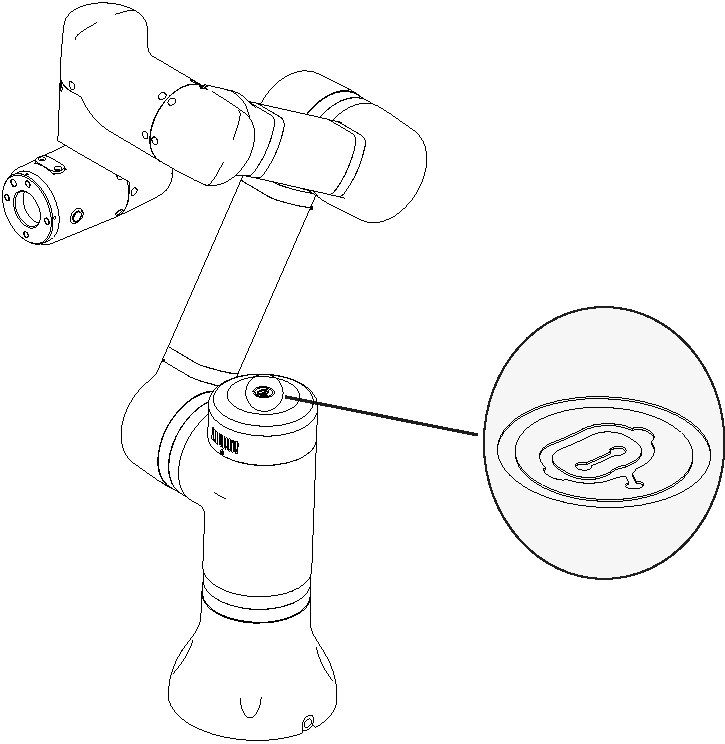
\includegraphics[height=6cm]{en/image/shoulder_btn.pdf}
	\caption{Shoulder button}
	\label{fig:肩部按钮示意图}
\end{figure}

\subsubsection{Robot Pose Safety Inspection}
When the current pose of the robot is the same as the first pose to be run\footnote{The first pose to be run: The chronologically first pose type action block in the set of action block that meets the conditions in the Timeline Editor (when no action block is selected, it refers to all the action blocks in the editor; when some action blocks are manually selected, it refers to these selected action blocks). This action block represents the first pose to be run. The robot control system will check the pose of the action block and compare it with the current pose of the robot.} in the scene, the scene runs without performing pose safety check. When the current pose of the robot is inconsistent with the first pose to be run in the scene, before running the scene, a pose safety check will be performed and the \nameref{fig:位置安全检查页} will pop up.

\begin{figure}[ht]
	\centering
	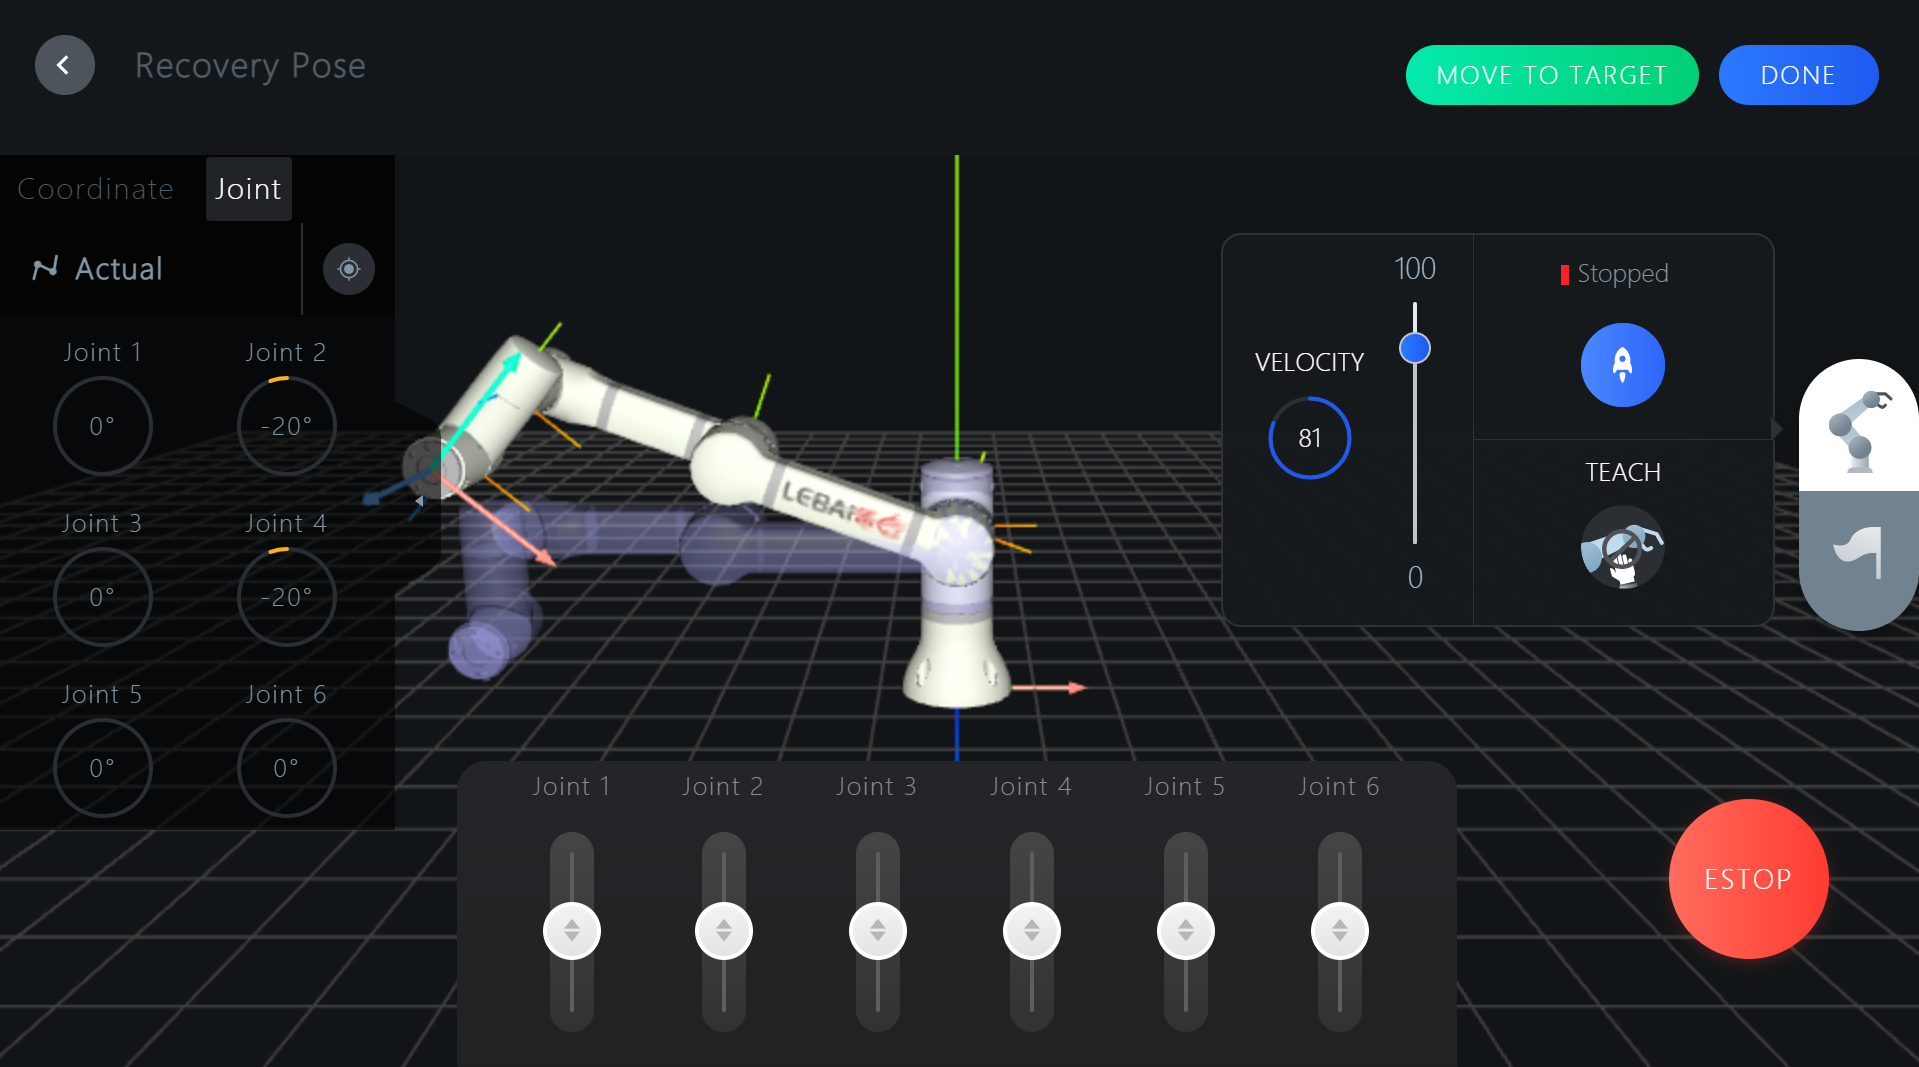
\includegraphics[width=\textwidth]{en/image/position_check.png}
	\caption{Restore pose window}
	\label{fig:位置安全检查页}
\end{figure}

In the Pose safety check window, there are two ways to move the robot to the first pose to be run in the scene:
\begin{itemize}
	\item Click the Pose safety check window to \\\btn[Success]{MOVE TO TARGET} and wait for the robot to move to the first pose to be run in the scene. You can click \btn[Danger]{STOP} at any time to stop the movement while moving.
	\item Long press the robot end flat button and release it after the robot moves to the first pose to be run in the task.
\end{itemize}

Click the \btn{Done} button in the upper right corner, and the scene starts to run. When the scene is running, long press the shoulder button to pause or resume a task.

\info{When the current pose of the robot is different from the first pose to be executed in the scene to be executed, pose safety check will be performed before the scene is executed.}

\danger[WARNING]{After using the flat end button to move the robot to the first pose to be run, please keep a safe distance from the robot and click the \btn{Done} button to run the scene, otherwise accidental injury might result.}

\subsection{Operation Skills}
\subsubsection{Quick Search Block}
Right­click a block and select \mnu{Find Similar Blocks} from the pop­up right­click menu to perform a quick search for blocks of the same block type and containing the currently selected block title as a keyword.
\subsubsection{Batch Edit Blocks}
% \def\ttt{通过搜索框或快速搜索动作块等操作或者手动选中}
% \def\ttt{通过选中}
% \ttt 2个或以上的同类型或子类型(如果该类型动作块存在子类型的话)相同的动作块。

\begin{figure}[htb]
	\centering
	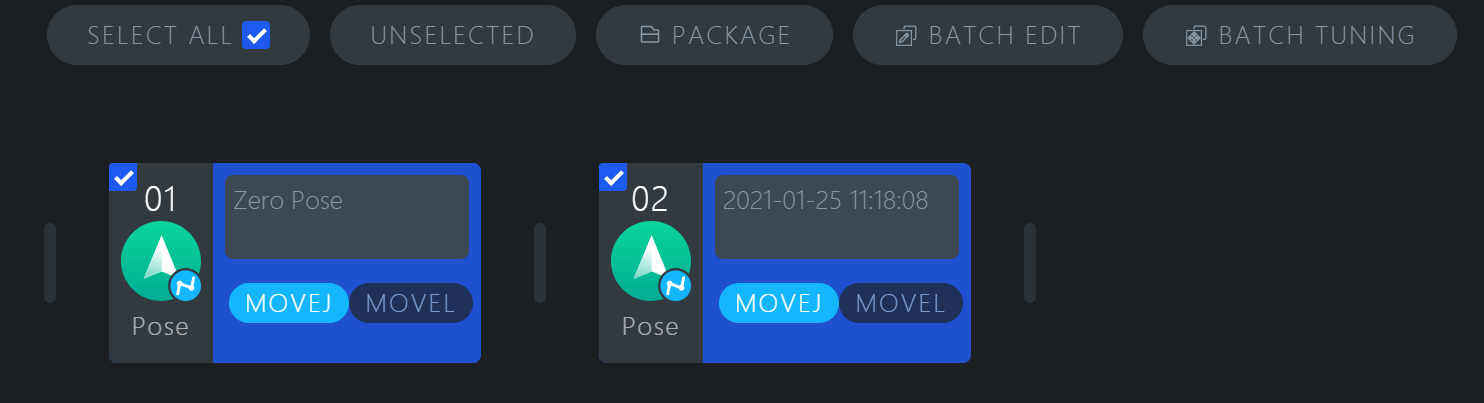
\includegraphics[width=\textwidth]{en/image/batch_adjust_positions.png}
	\caption{Batch Edit Blocks}
	\label{fig:批量编辑动作块}
\end{figure}

Click the \btn[Info]{BATCH EDIT} button in the functional area of the scene editor, or right­click the block and select \mnu{Batch Edit} to edit the following contents of the block in batches.

\begin{itemize}[leftmargin=7.5em]
\item [Pose Block] You can uniformly edit the pose name, switch between joint space movement (movej) and Cartesian space linear movement (movel), speed and acceleration time, and enable and disable smoothing functions. After confirming the batch modification, the data of every individual pose block will be updated with the pose data of the robot in the current state.
\item [Gripper Block] The description, strength and amplitude of the Gripper action can be modified.
\item [Waiting Block] The number of seconds to wait and the description of the purpose/function of the wait can be modified.
\item [Notification Block] The light board prompt and pop­up prompt are different sub­types of blocks, and different sub­types of blocks cannot be modified in batches.
\item [Digital I/O Block] Support batch modification of reading, waiting and setting.
\item [Analog I/O Block] Support batch modification of reading, waiting and setting.
\item [Payload Block] Support batch modification of load quality or CoG of blocks of the same subtype.
\end{itemize}

Click the \btn{EDIT} button in the lower right corner of the dialog box to perform batch editing operation. You can click the \kbd{$\times$} button in the upper right corner to cancel the operation.

\info{For batch editing of blocks, the block type and subtype (if there are subtypes for this type of blocks) must be consistent.}

% \clearpage

\subsubsection{Batch Fine-Tuning of Pose Blocks}
Select 2 or more pose blocks, and click the \btn[Info]{Batch Tuning} in the functional area of the Timeline Editor or place the cursor on the selected pose block so that the current pose block is in focus, then right­click and select \mnu{Batch fine adjustment position} in the pop-up menu to enter the \mnu{Adjustment position} page\footnote{See \prettyref{sec:微调}.}.

\begin{figure}[hb]
	\centering
	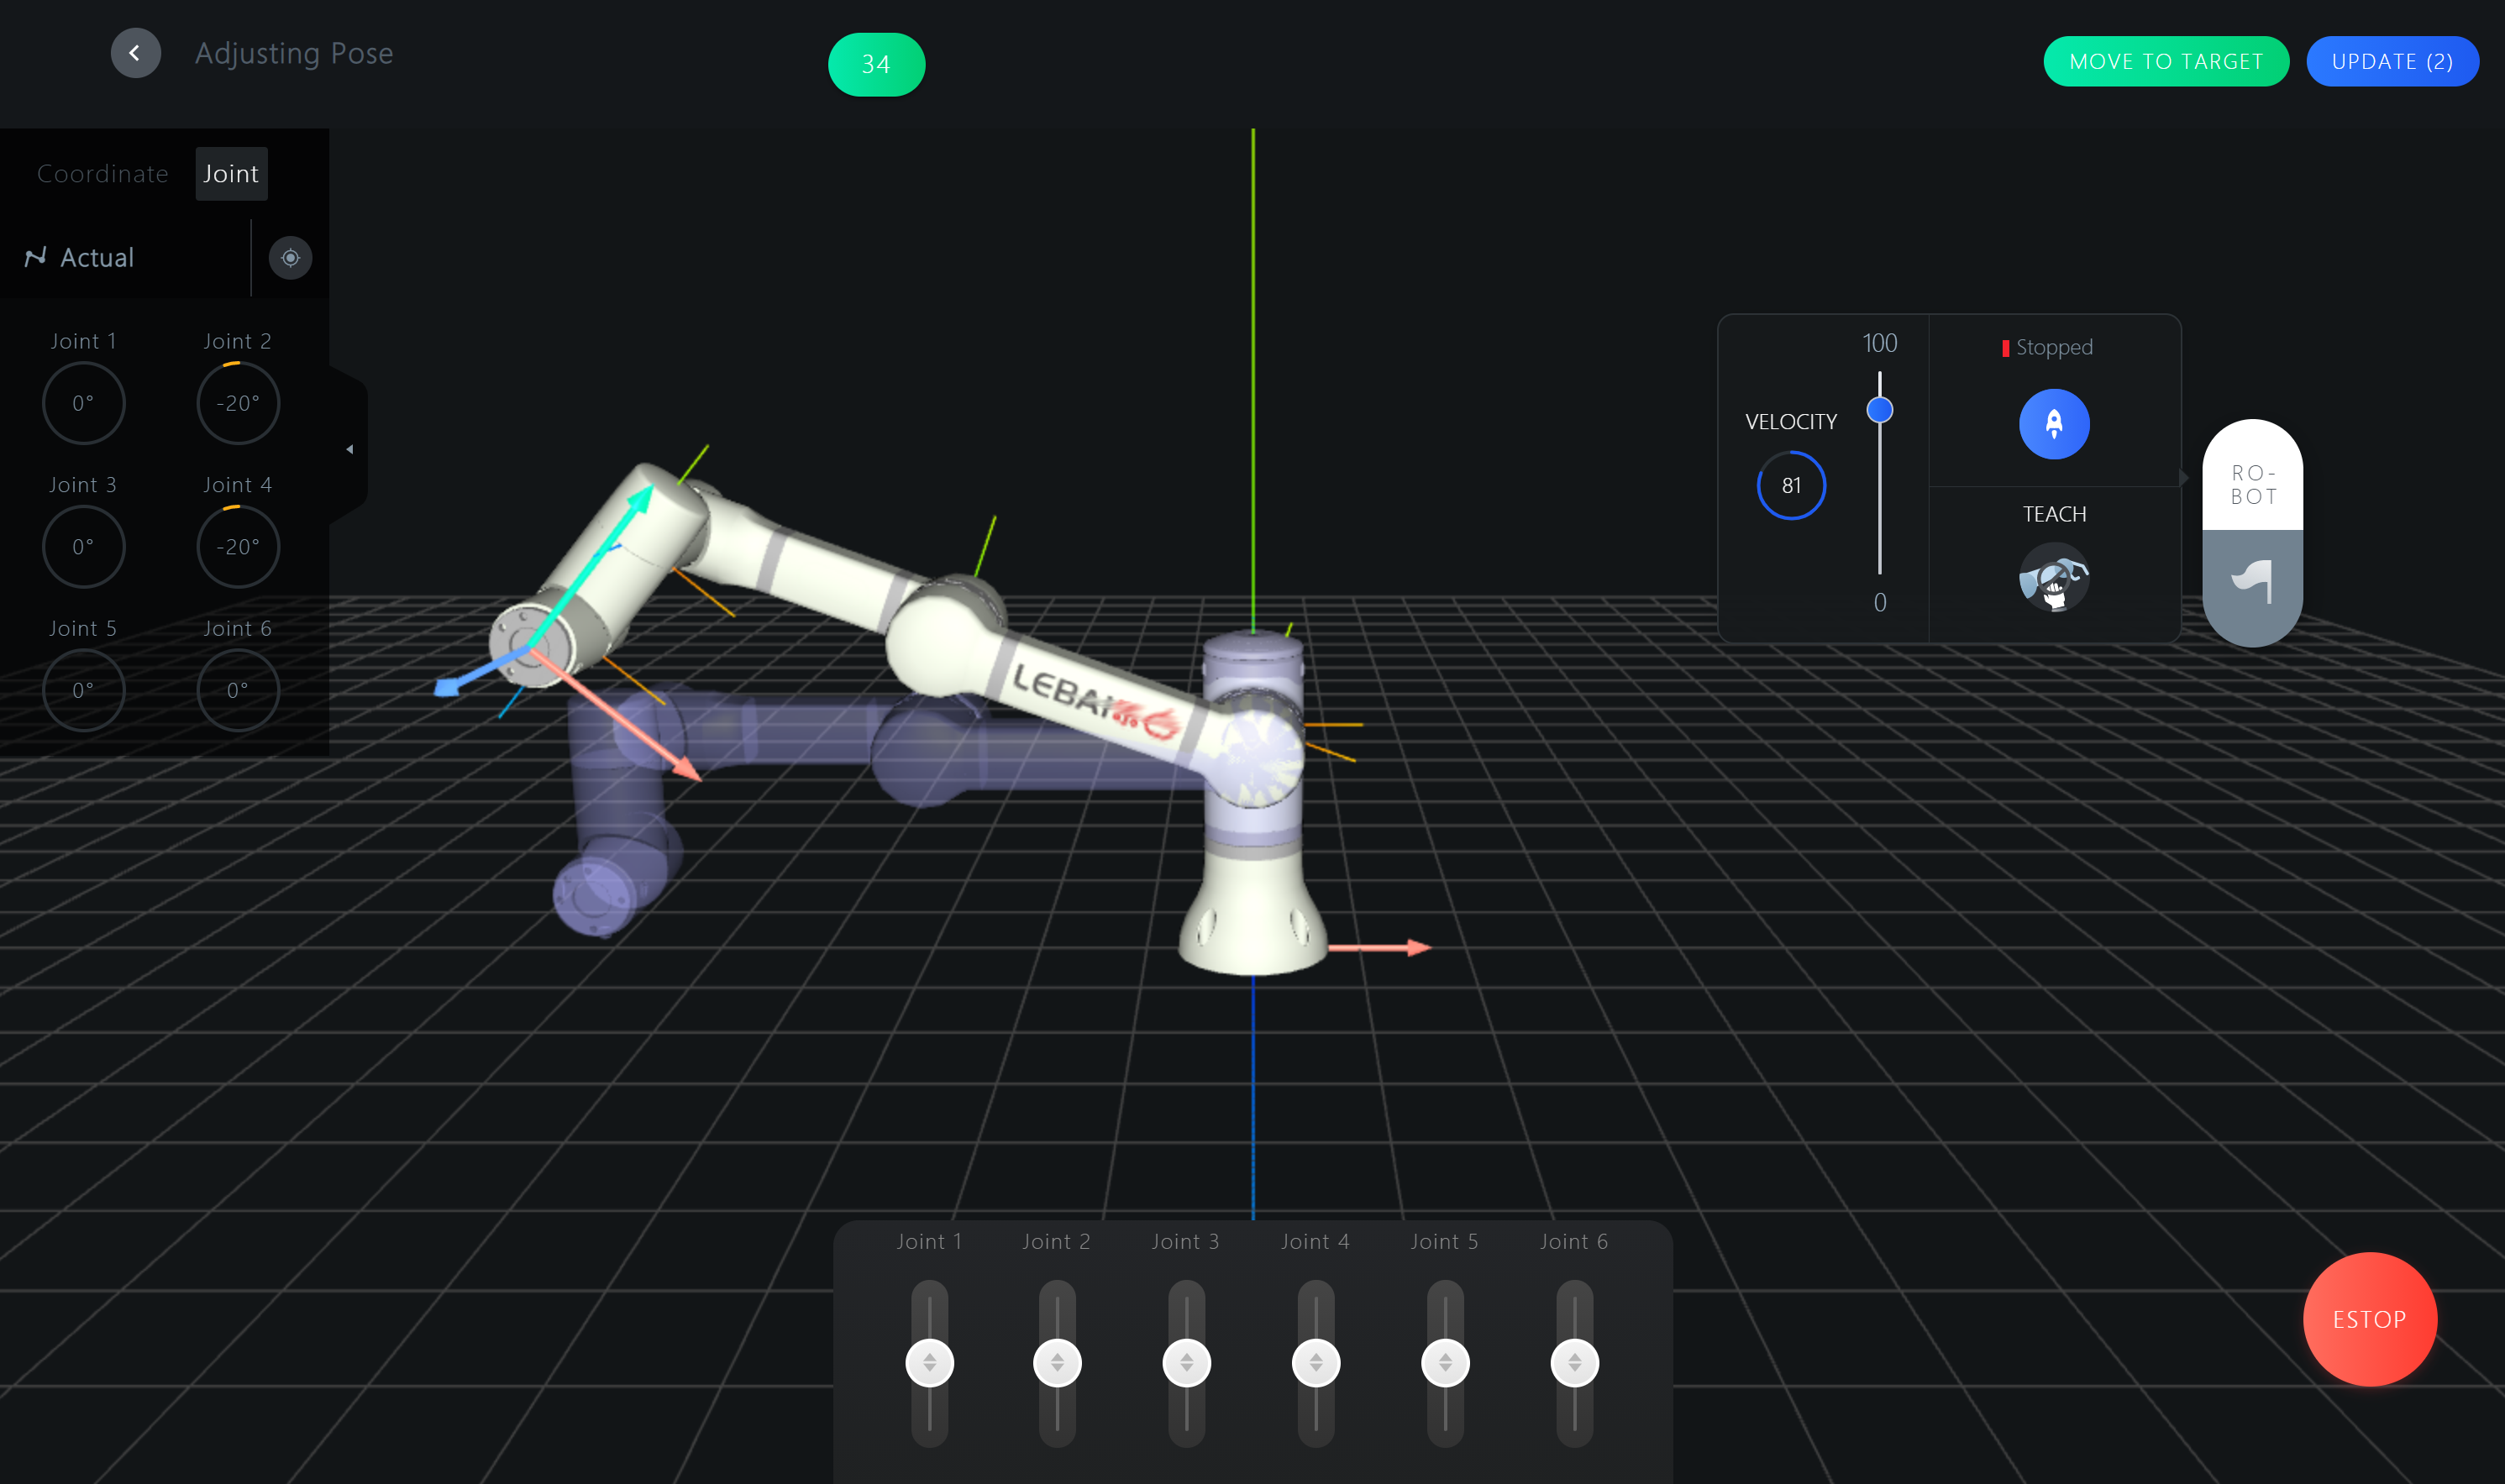
\includegraphics[width=\textwidth]{en/image/poses.png}
	\caption{Batch Fine-Tuning of Pose Blocks}
	\label{fig:批量微调位置块}
\end{figure}

After the fine­tuning to the target position, you can click the \btn{UPDATE} button in the upper right corner of the page to complete the batch fine­tuning or click \btn[Info]{CANCEL} to abandon the batch fine­tuning operation. The number on the right side of the \btn{UPDATE} button indicates the total number of currently selected location blocks.

\clearpage

\subsection{Export Scene}
\label{sec:导出场景}
Select the scene to be saved on the scene list page, and move the mouse to the \icn{image/vdots.pdf} button in the upper right corner of the scene card to pop up the scene menu. Select \mnu{Export}, then choose a save location of the scene file in the pop­up save dialog box (the file extension is \verb|lbd|).

\begin{figure}[htb!]
	\centering
	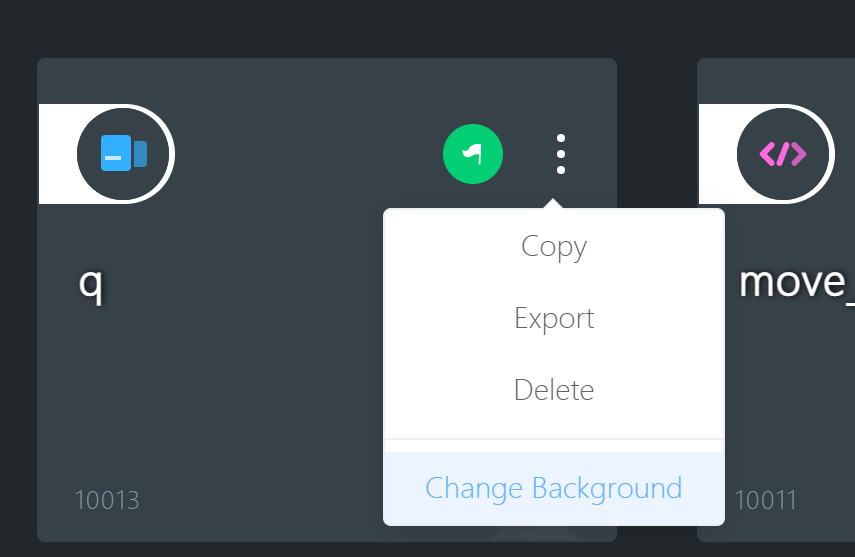
\includegraphics[height=3cm]{en/image/3-19.png}
	\caption{Export Scene}
	\label{fig:导出场景}
\end{figure}

\subsection{Import Scene}
\label{sec:导入场景}
As shown in \prettyref{fig:导入场景}, in the toolbar of the \mnu{scene list}, click \icn{image/icon_import.pdf} icon to open the scene file you exported. After the import is complete, the scene will be introduced automatically.

\begin{figure}[htb!]
	\centering
	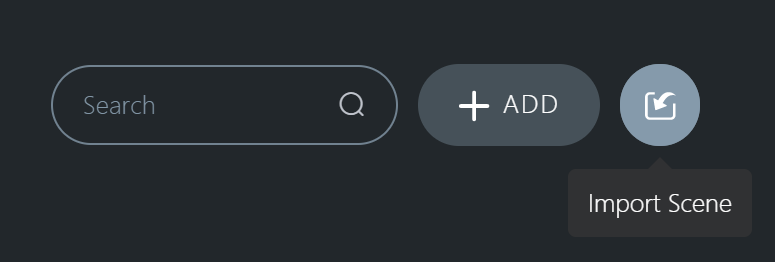
\includegraphics[height=1.8cm]{en/image/3-20.png}
	\caption{Import Scene}
	\label{fig:导入场景}
\end{figure}

% \clearpage

\section{Control}
The control module is mainly divided into:
\begin{itemize}
\item Virtual Control
\item Pose Library
\item I/O Control
\item Gripper Control
\item Hardware Button
\item LED Control
\end{itemize}

\subsection{Virtual Control}
The current pose of the robot can be adjusted through virtual control.  Refer to the introduction of fine­tuning function in \\\prettyref{sec:微调} for specific operation methods.

\begin{figure}[ht]
	\centering
	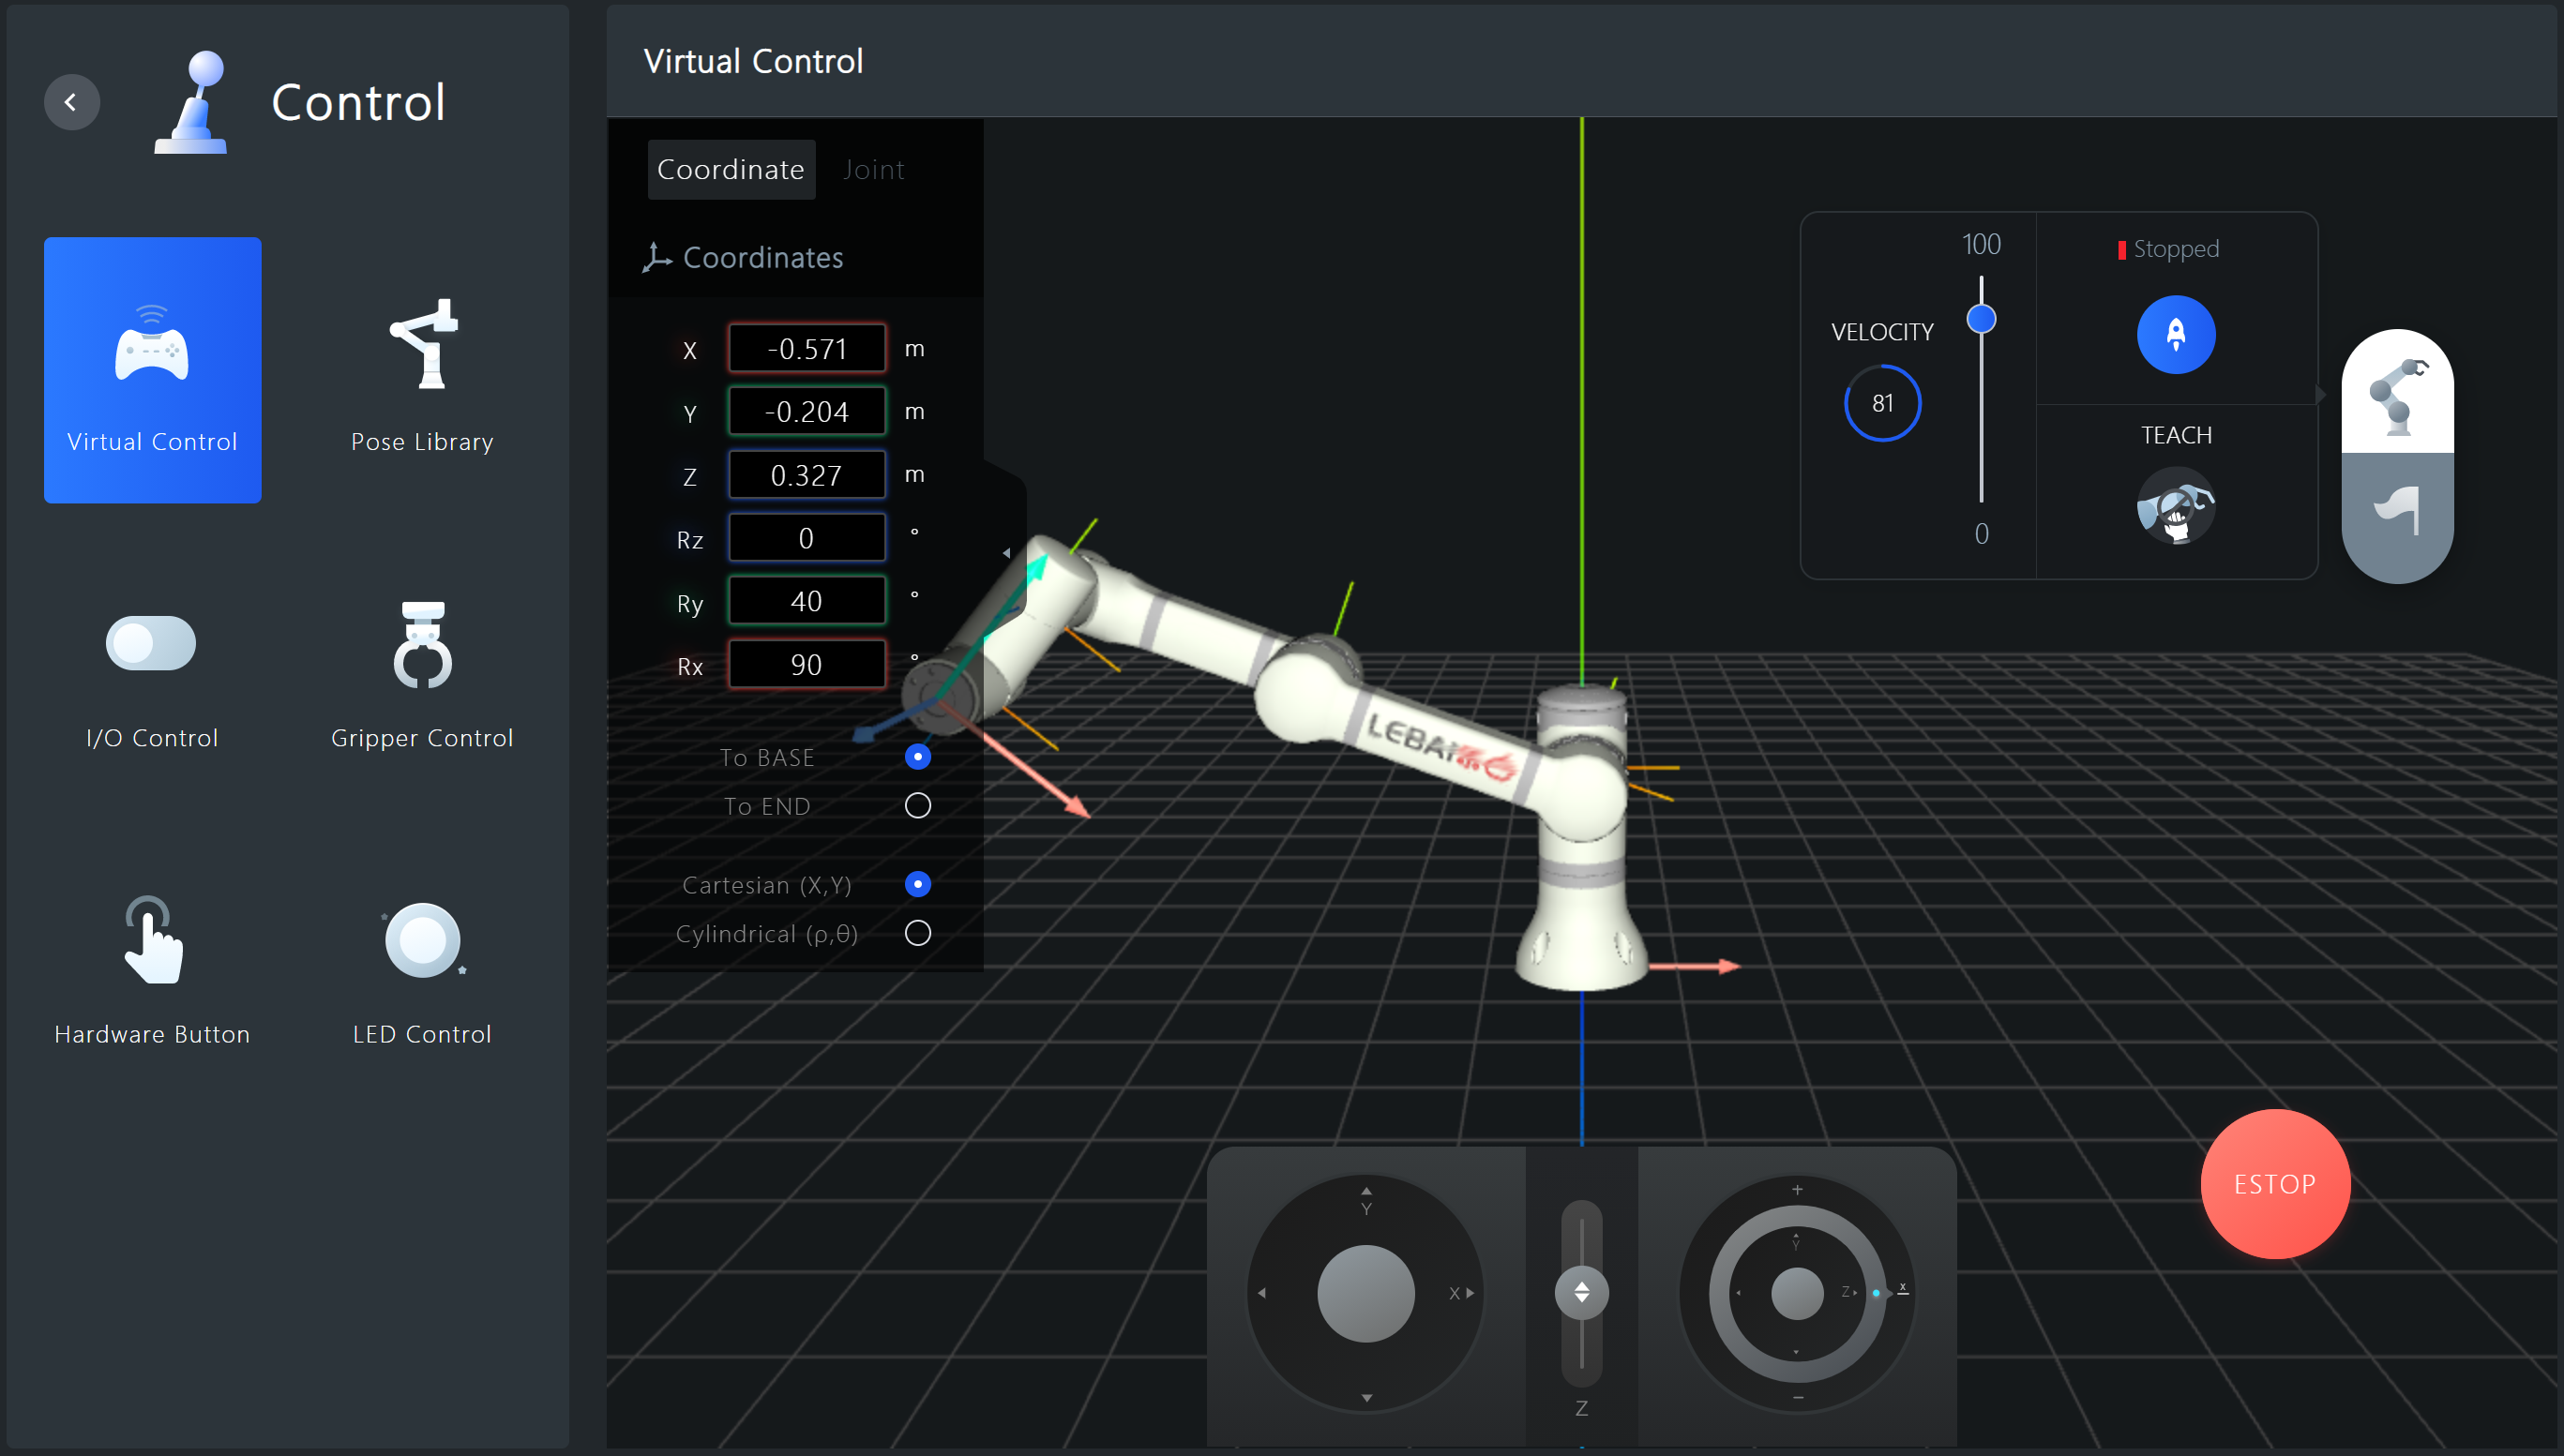
\includegraphics[width=\textwidth]{en/image/3-21.png}
	\caption{Virtual control}
	\label{fig:虚拟控制示意图}
\end{figure}

\subsection{Hardware button}
\label{sec:硬件按钮}

\begin{figure}[ht]
	\centering
	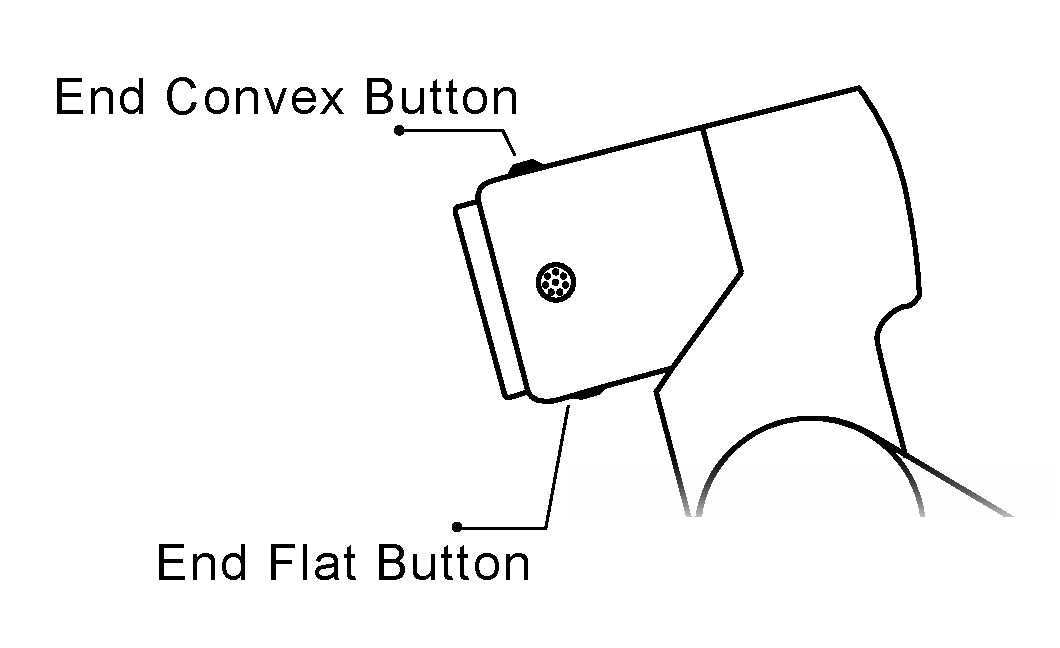
\includegraphics[height=3cm]{en/image/flange_buttons.pdf}
	\caption{Flange buttons}
	\label{fig:末端按钮示意图}
\end{figure}

\begin{enumerate}[label=(\arabic*)]
	\item The robot's end flat button
	\begin{itemize}
		\item[Click] The timeline editing focus moves backward by one block;
		\item[Double-click] The timeline editing focus moves forward by one block;
		\item[Long press] If you are currently at the pose block's Refresh pose pop­up box (click the fine­tuning button of the pose block to enter) or the pose library's Apply pose pop­up box, move to the target position;
		\item[Release] When moving to the target pose after a long press, release the button will stop the current movement.
	\end{itemize}

	\item The robot's end convex button
	\begin{itemize}
		\item[Long press] Enter the teaching mode;
		\item[Release] Exit the teaching mode;
		\item[Double click] Add a pose block/code in the editor;
		\item[Click] Only if that the current block is a pose block, when the current pose block is not in the fine adjustment pose dialog box, click this button to enter the fine adjustment current pose dialog box. If the current pose block is already in the fine adjustment pose dialog box, you can click this button to update the pose data saved in the current block.
	\end{itemize}

	\item Shoulder button
	\begin{itemize}
		\item[Long press] Switch between queue pause and resume, i.e., pause when \mnu{RUNNING} or resume when \mnu{PAUSED};
		\item[Click] When there is a popup or other secondary interface in the scene editor, cancel the operation (button, dialog box, etc.);
		\item[Double-click] If you are currently in the scene editor interface and there is no other pop­up box, switch between run and stop operation; otherwise, confirm the operation (button, dialog box, etc.).
	\end{itemize}

	\item Button combo
	\begin{itemize}
		\item [Start/stop] Long press the flat button at the end of the robot then press the shoulder button at the same time to switch between starting and stopping the robot.

	\end{itemize}
\end{enumerate}
		\info{The button combo for starting/stopping the robot is only available when the robot is not in emergency stop state or not powered off.}

\section{Device}
\subsection{End Device}
\label{sec:末端设备}
If you need to add a effector (such as a gripper) at the end of the robot, first click \mnu{DEVICE}; then click \btn{ADD} on the end device to set the mass and CoG of the corresponding auxiliary tool; and finally, click \mnu{Enable}. If you need to remove the end effector, click \mnu{Disable}.

\danger[WARNING]{\begin{itemize}
	\item The mass and CoG should be as consistent as possible with the mass and CoG of the end effector added.
	\item When replacing or removing the end effector, be sure to edit the mass and CoG of the end device ac­ cordingly or close the corresponding end device, otherwise accidental injury might result.
\end{itemize}}

\section{Settings}
\subsection{TCP Settings}
\label{sec:TCP设置}
The full name of TCP is Tool Center Point, which means the center point of the robot tool. You can use the TCP setting page to set the offset/conversion amount of the TCP pose and posture of the robot end. The system does not set TCP by default. When the an end effector is installed on the robot, you may choose to add TCP settings according to the scene application.

TCP can be added by teaching. Click the \btn{ADD} button, the \mnu{Teaching Add} in the menu, open the \nameref{fig:示教添加TCP设置} to add TCP settings, as shown in \prettyref{fig:示教添加TCP设置}. Now you can click the Teaching icon and drag-and-drop teach the robot to confirm the four key points one by one in four different postures while the end effector of the robot touches the same control point (that is, keeps the end effector always in contact with the same position). The robot can automatically recognize the TCP pose information according to the different positions and directions of the end flange. The posture information does not support ``add by teaching'' currently, thus need to be filled out manually.

\begin{figure}[htb]
	\centering
	\begin{minipage}[t]{0.48\linewidth}
		\centering
		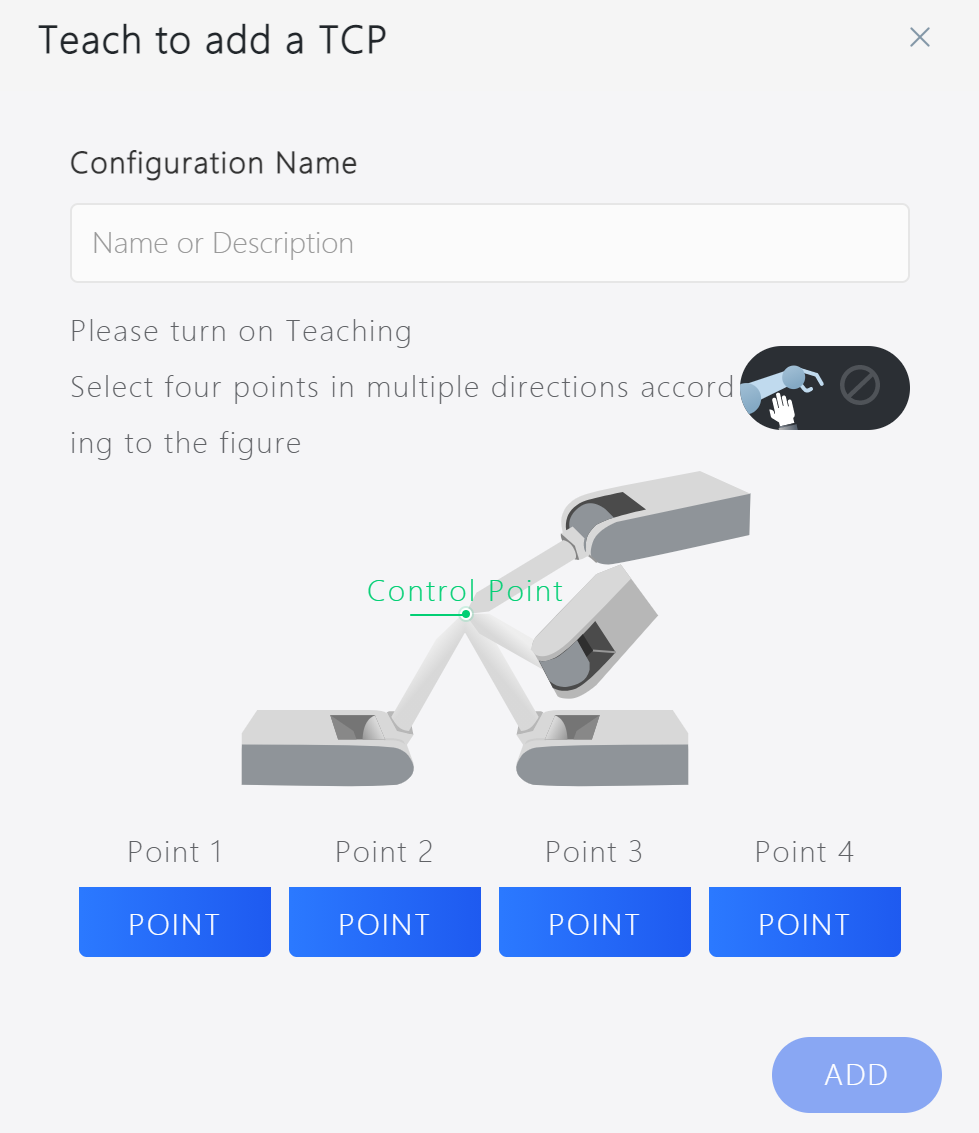
\includegraphics[width=\linewidth]{en/image/3-24.png}
		\caption{Add TCP settings by teaching}
		\label{fig:示教添加TCP设置}
	\end{minipage}
	\hfill
	\begin{minipage}[t]{0.48\linewidth}
		\centering
		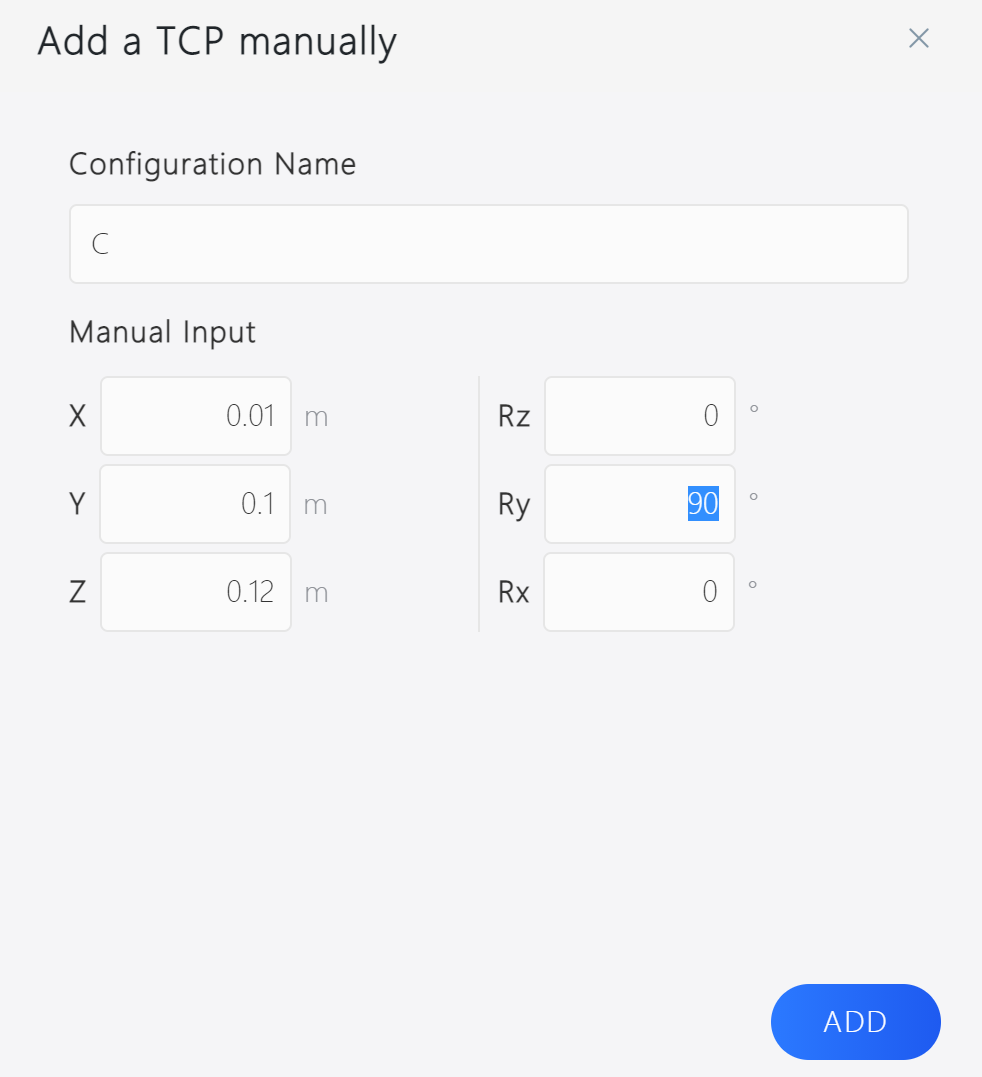
\includegraphics[width=\linewidth]{en/image/3-25.png}
		\caption{Edit TCP settings}
		\label{fig:编辑TCP设置}
	\end{minipage}
\end{figure}

As shown in \prettyref{fig:编辑TCP设置}, the user can also \mnu{Add} or \btn[Card]{EDIT} to enter the \nameref{fig:编辑TCP设置} settings and set the pose and posture of the end effector manually.

% \vfill

\subsection{Safe Settings}
\subsubsection{Collision detection}
The default state of the robot collision detection is \mnu{Emergency Stop} after the installation guide is opened. While operating, the robot's actions after detecting a collision with external resistance are divided into two types: \mnu{Pause} and \mnu{Emergency Stop}. You can adjust the detection sensitivity by yourself.

\begin{figure}[htb]
	\centering
	\subfigure[Emergency Stop]{\begin{minipage}[t]{0.48\linewidth}
		\centering
		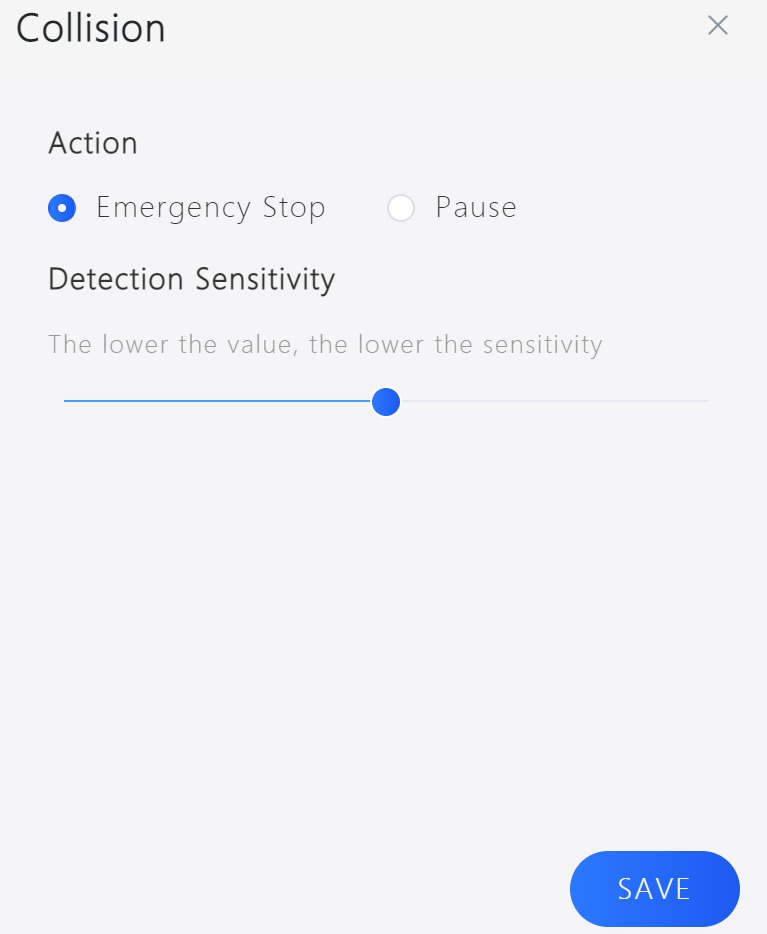
\includegraphics[width=\linewidth]{en/image/3-26-1.png}
	\end{minipage}}
	\hfill
	\subfigure[Pause]{\begin{minipage}[t]{0.48\linewidth}
		\centering
		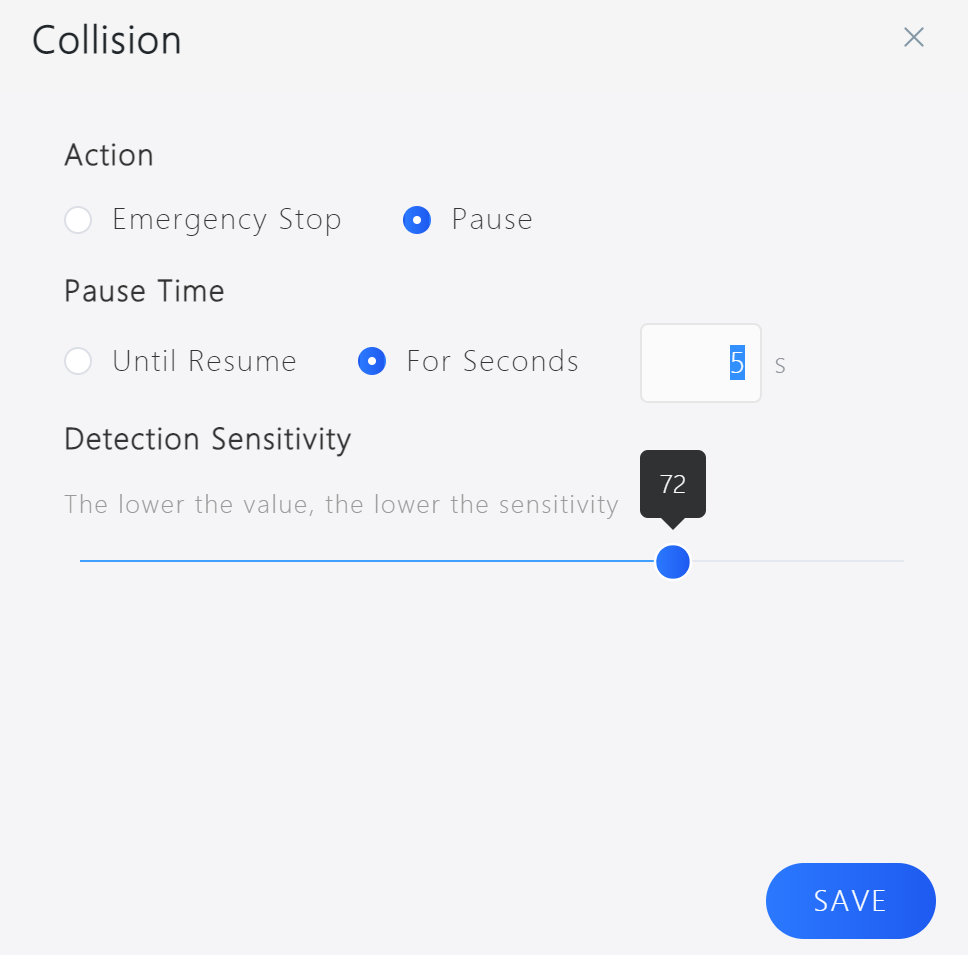
\includegraphics[width=\linewidth]{en/image/3-26-2.png}
	\end{minipage}}
	\caption{Collision detection}
	\label{fig:碰撞检测设置}
\end{figure}

Action after collision:
\begin{description}%[leftmargin=8cm]
	\item[Emergency Stop] In this case, the robot needs to be restarted and taught to a safe pose before continuing the operation.
	\item[Pause] If you select a custom number of seconds, the task will automatically resume when the specified pause time is reached; if you select permanent pause, you need to click the Resume task button \icn{image/39.pdf} in the task history list column on the homepage.
\end{description}

% \newpage

\subsubsection{Operational Safety}
\label{sec:运行安全}
In operational safety, you can view and adjust the following runtime parameters:
\begin{itemize}
	\item Maximum and minimum angle of each joint
	% \item 在关节空间运行时的最大速度和最大加速度限制
	% \item 在坐标空间运行时的最大速度和最大加速度限制
	\item Joint space operation configuration
	\item Coordinate space running configuration
\end{itemize}

% 其中,关节空间运行时的最大速度和最大加速度限制应用于场景编辑在时间轴编辑器模式下,使用滑杆调整速度和加速时间(加速度)时的最大值,控制系统限制关节空间相关移动(movej)的速度和加速度的最大值以及全局限定每个关节运行时的最大速度限制时有效。当任意一个关节运行时的速度超过最大速度限制时,机器人会自动急停。

% 坐标空间运行时的最大速度和最大加速度限制应用于场景编辑器在时间轴编辑器下,使用滑杆调整速度加速时间(加速度)时的最大值以及控制系统限制坐标空间相关移动(movel, movec)的速度和加速度的最大值。

\begin{figure}[htb!]
	\centering
	% 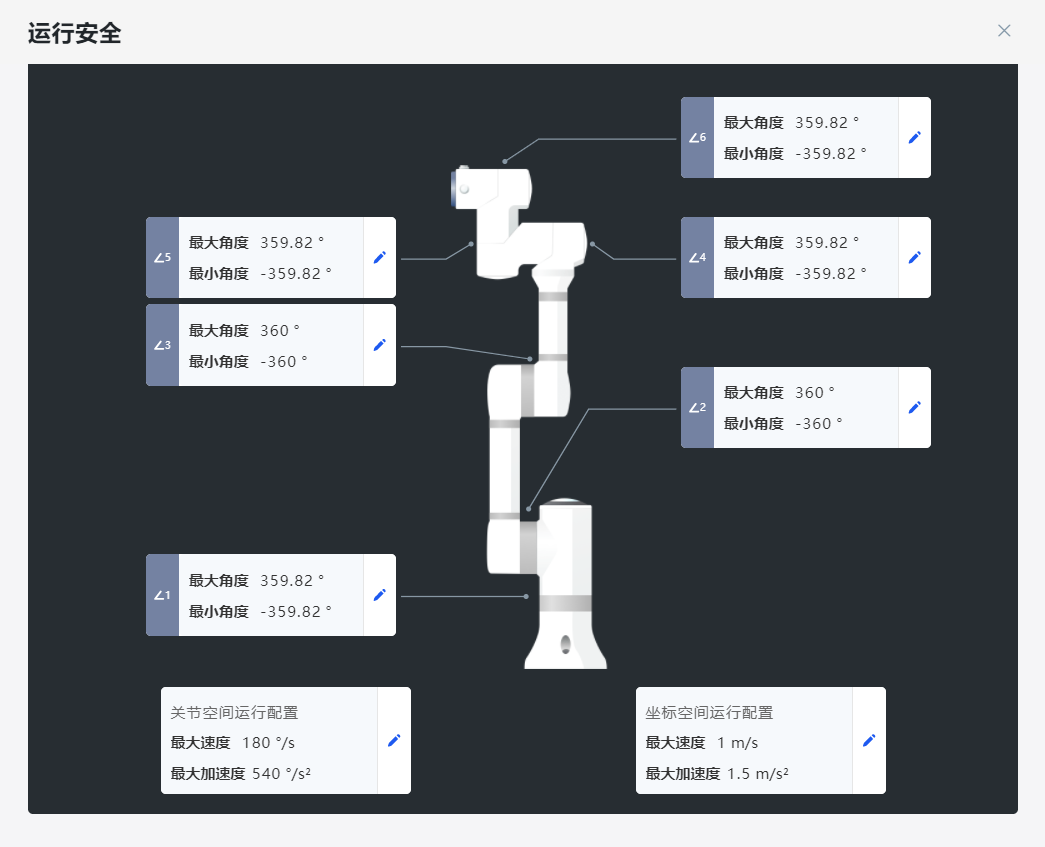
\includegraphics[height=7.5cm]{en/image/3-27.png}
	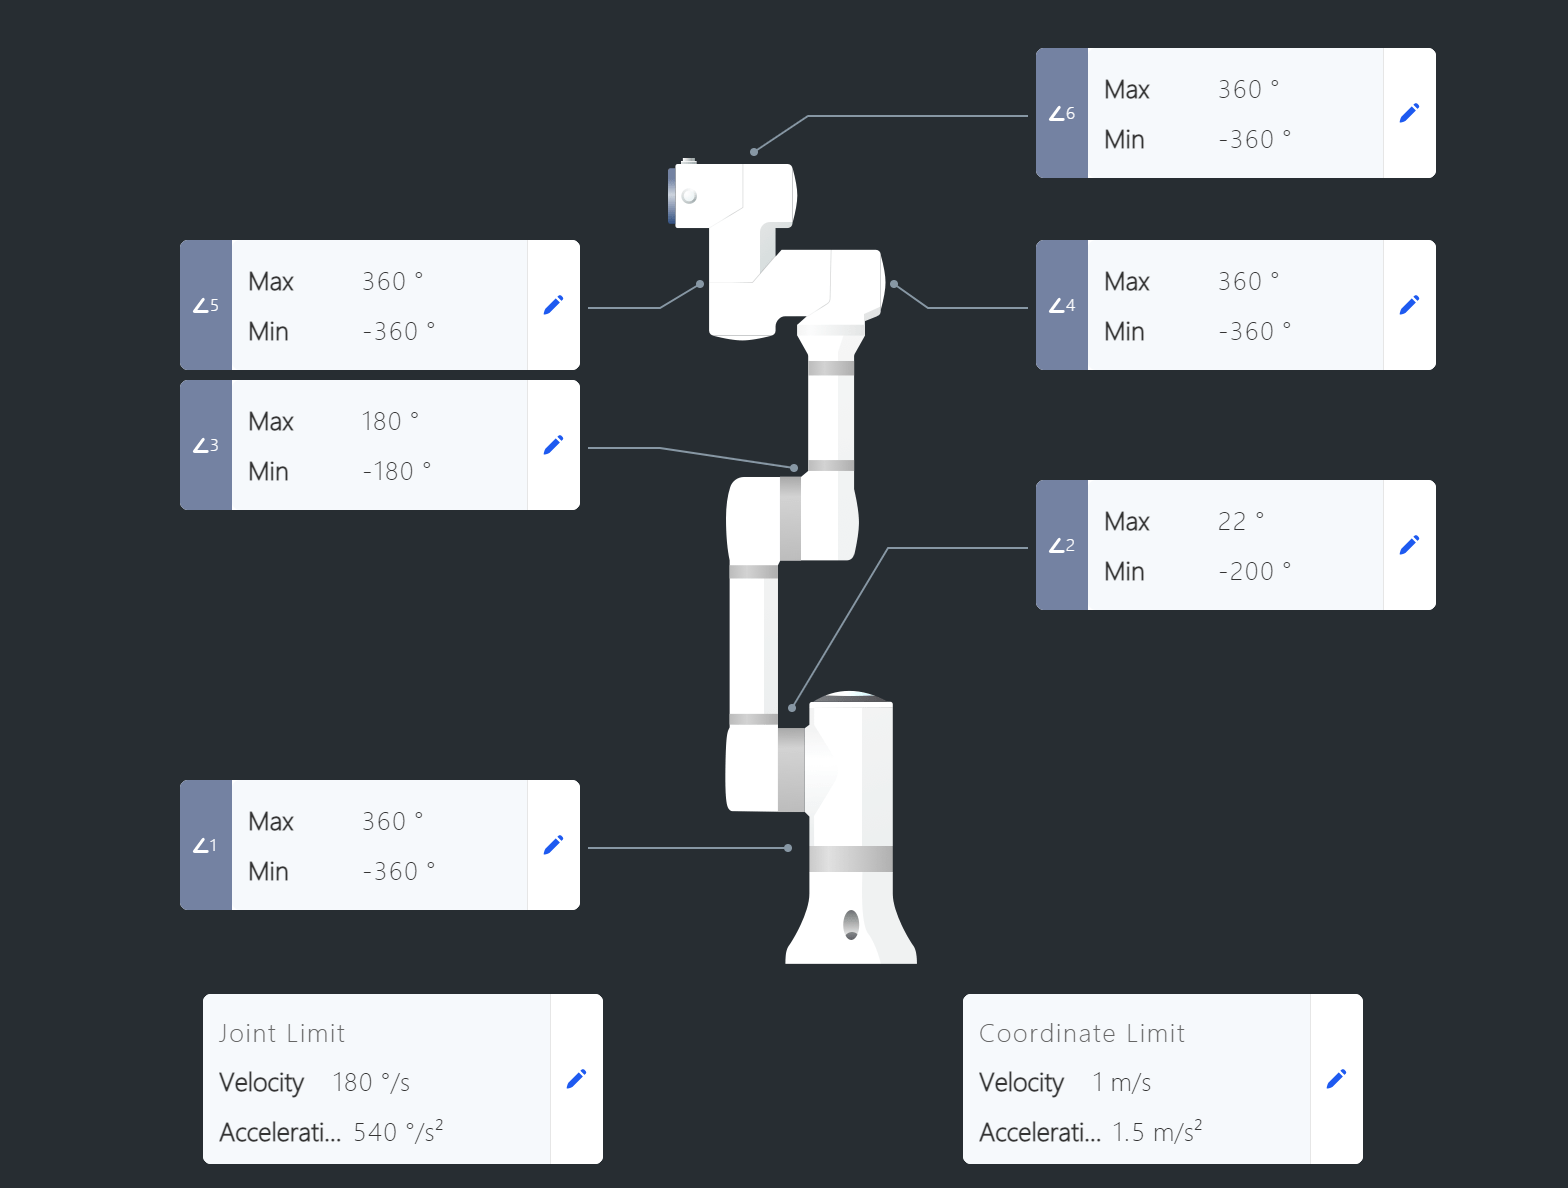
\includegraphics[height=7.5cm]{en/image/safe.png}
	\caption{Operation safety settings}
	\label{fig:运行安全设置}
\end{figure}

% \info{关节的最小角度和最大角度理论上可以设置为任意值。建议使用出厂时预置的默认值(如\prettyref{fig:运行安全设置})。
% % 如需调整,为了编程和调试方便,用户可以设置为$-360\sim 360^\circ$。
% }

\info{Editing the running configuration of the robot's joint space will affect the robot's speed limit. When the running speed of any joint exceeds the maximum speed limit, the robot will emergency stop automatically.}

\danger{Editing the running configuration of the robot joint space and editing the running configuration of the coordinate space will affect the speed and acceleration time (acceleration) of the pose block in the scene editor proportionally.}

% \danger[警告]{非专业用户在不确定修改后的风险情况下,不可随意更改。}

% \clearpage

\subsection{Operation mode}
There are two operating modes as follows for you to choose according to your own situation:
\paragraph{Normal Mode}
In the beginner mode you can use the easy-to-use Timeline Editor. Some functions of the expert mode will be hidden in the beginner mode to save you the trouble brought by complex and advanced functions.
\paragraph{Expert Mode}
% 专家模式使用专业代码编辑器。
In expert mode:
\begin{itemize}
\item You can switch to Code Editor which uses Lua as the programming language.
\item You can convert scenes in the Timeline Editor into Lua codes.
\item You can close the pose safety check in the Timeline Editor mode.
\item Supports installation settings and can customize the configuration of any install direction.
\end{itemize}

\info{Before closing the safety check, please make sure that you are well aware of the danger of the operation.}

% \vfill

To switch between operation modes:
\begin{itemize}
	\item Enter the \mnu{SETTING} page, perform switchovers in the \\\mnu{OPERATION MODE} and save the operation.
	\item Click the switch icon in the upper right corner of the scene editing page to switch and save the operation mode.
\end{itemize}

% \vfill

% \clearpage

\subsection{System update}

Enter the \mnu{SETTINGS}, on the \mnu{SYSTEM UPDATE} page, if the current system is up to date, the icon in the center of the screen will be blue, as shown in \prettyref{fig:系统更新}. Click \btn{CHECK SYSTEM}, the circular pattern in the center of the screen shows \mnu{Checking for Updates}.

\begin{figure}[htb]
	\centering
	\subfigure[The current system is up to date]{\begin{minipage}[t]{0.3\linewidth}
		\centering
		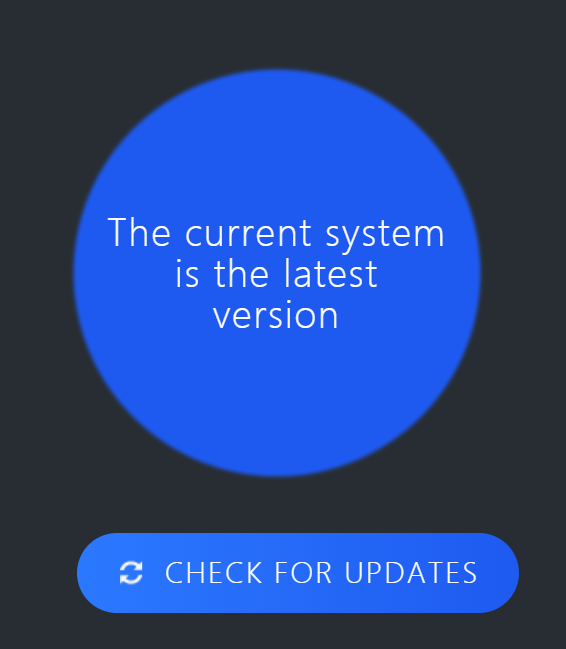
\includegraphics[width=\linewidth]{en/image/3-28.png}
	\end{minipage}}
	\qquad
	\subfigure[Available update detected]{\begin{minipage}[t]{0.3\linewidth}
		\centering
		
\includegraphics[width=\linewidth]{en/image/3-29.png}
	\end{minipage}}
	\caption{System update}
	\label{fig:系统更新}
\end{figure}

When an available update of the system is detected, the icon in the center of the screen turns orange and displays ``System update detected'' with latest version number found. Click \btn[Warning]{Update} below, and the system will automatically update to the latest version.

\info{\begin{itemize}
	\item Please make sure that the robot status is \mnu{STOPPED} before updating the system.
	\item During system update, no other operations are allowed, otherwise serious consequences such as damage to the robot system may result.
\end{itemize}}
